\documentclass[a4paper,12pt]{book}
\usepackage[utf8]{inputenc}
\usepackage{graphicx}
\usepackage{caption}
\usepackage{subcaption}
\graphicspath{ {./screen_shots/} }
\usepackage{hyperref}
\usepackage{float}

\begin{document}

\author{}
\title{MANUAL v0.25}
\date{\today}

\frontmatter
\maketitle
\tableofcontents

\mainmatter

\chapter{Introduction}
This manual v0.25 is prepared for mobile mapping system \url{https://github.com/JanuszBedkowski/mandeye_controller/blob/main/doc/manual/manual_v0_1/mandeye_dev_manual_v0_1.pdf}{MANDEYE} available as open hardware project.
The software is composed of:
\begin{itemize}
	\item Lidar odometry (for initial trajectory calculation),
	\item Multi view terrestrial laser scan registration (for final trajectory calculation).
\end{itemize}
To use the software click the link below:

\url{https://github.com/MapsHD/HDMapping/releases}
\linebreak
and download the latest version of files: laszip3.dll, \verb|lidar_odometry_step_1.exe|, \verb|multi_session_registration_step_3.exe|  and \verb|multi_view_tls_registration_step_2.exe|.
Then put all of the downloaded files in one folder and proceed to next chapter.





\chapter{Lidar odometry}
This software calculates trajectory based on Lidar and IMU data.
It based on novel approach that I did not have opportunity to publish (work in progress).
Basically it is SAM (Smoothing and Mapping) approach that is using multi view Normal Distributions Transform in pose graph SLAM framework writen from scratch in Python (SymPy) and C++ (Eigen).
 

\begin{figure}
	\centering
	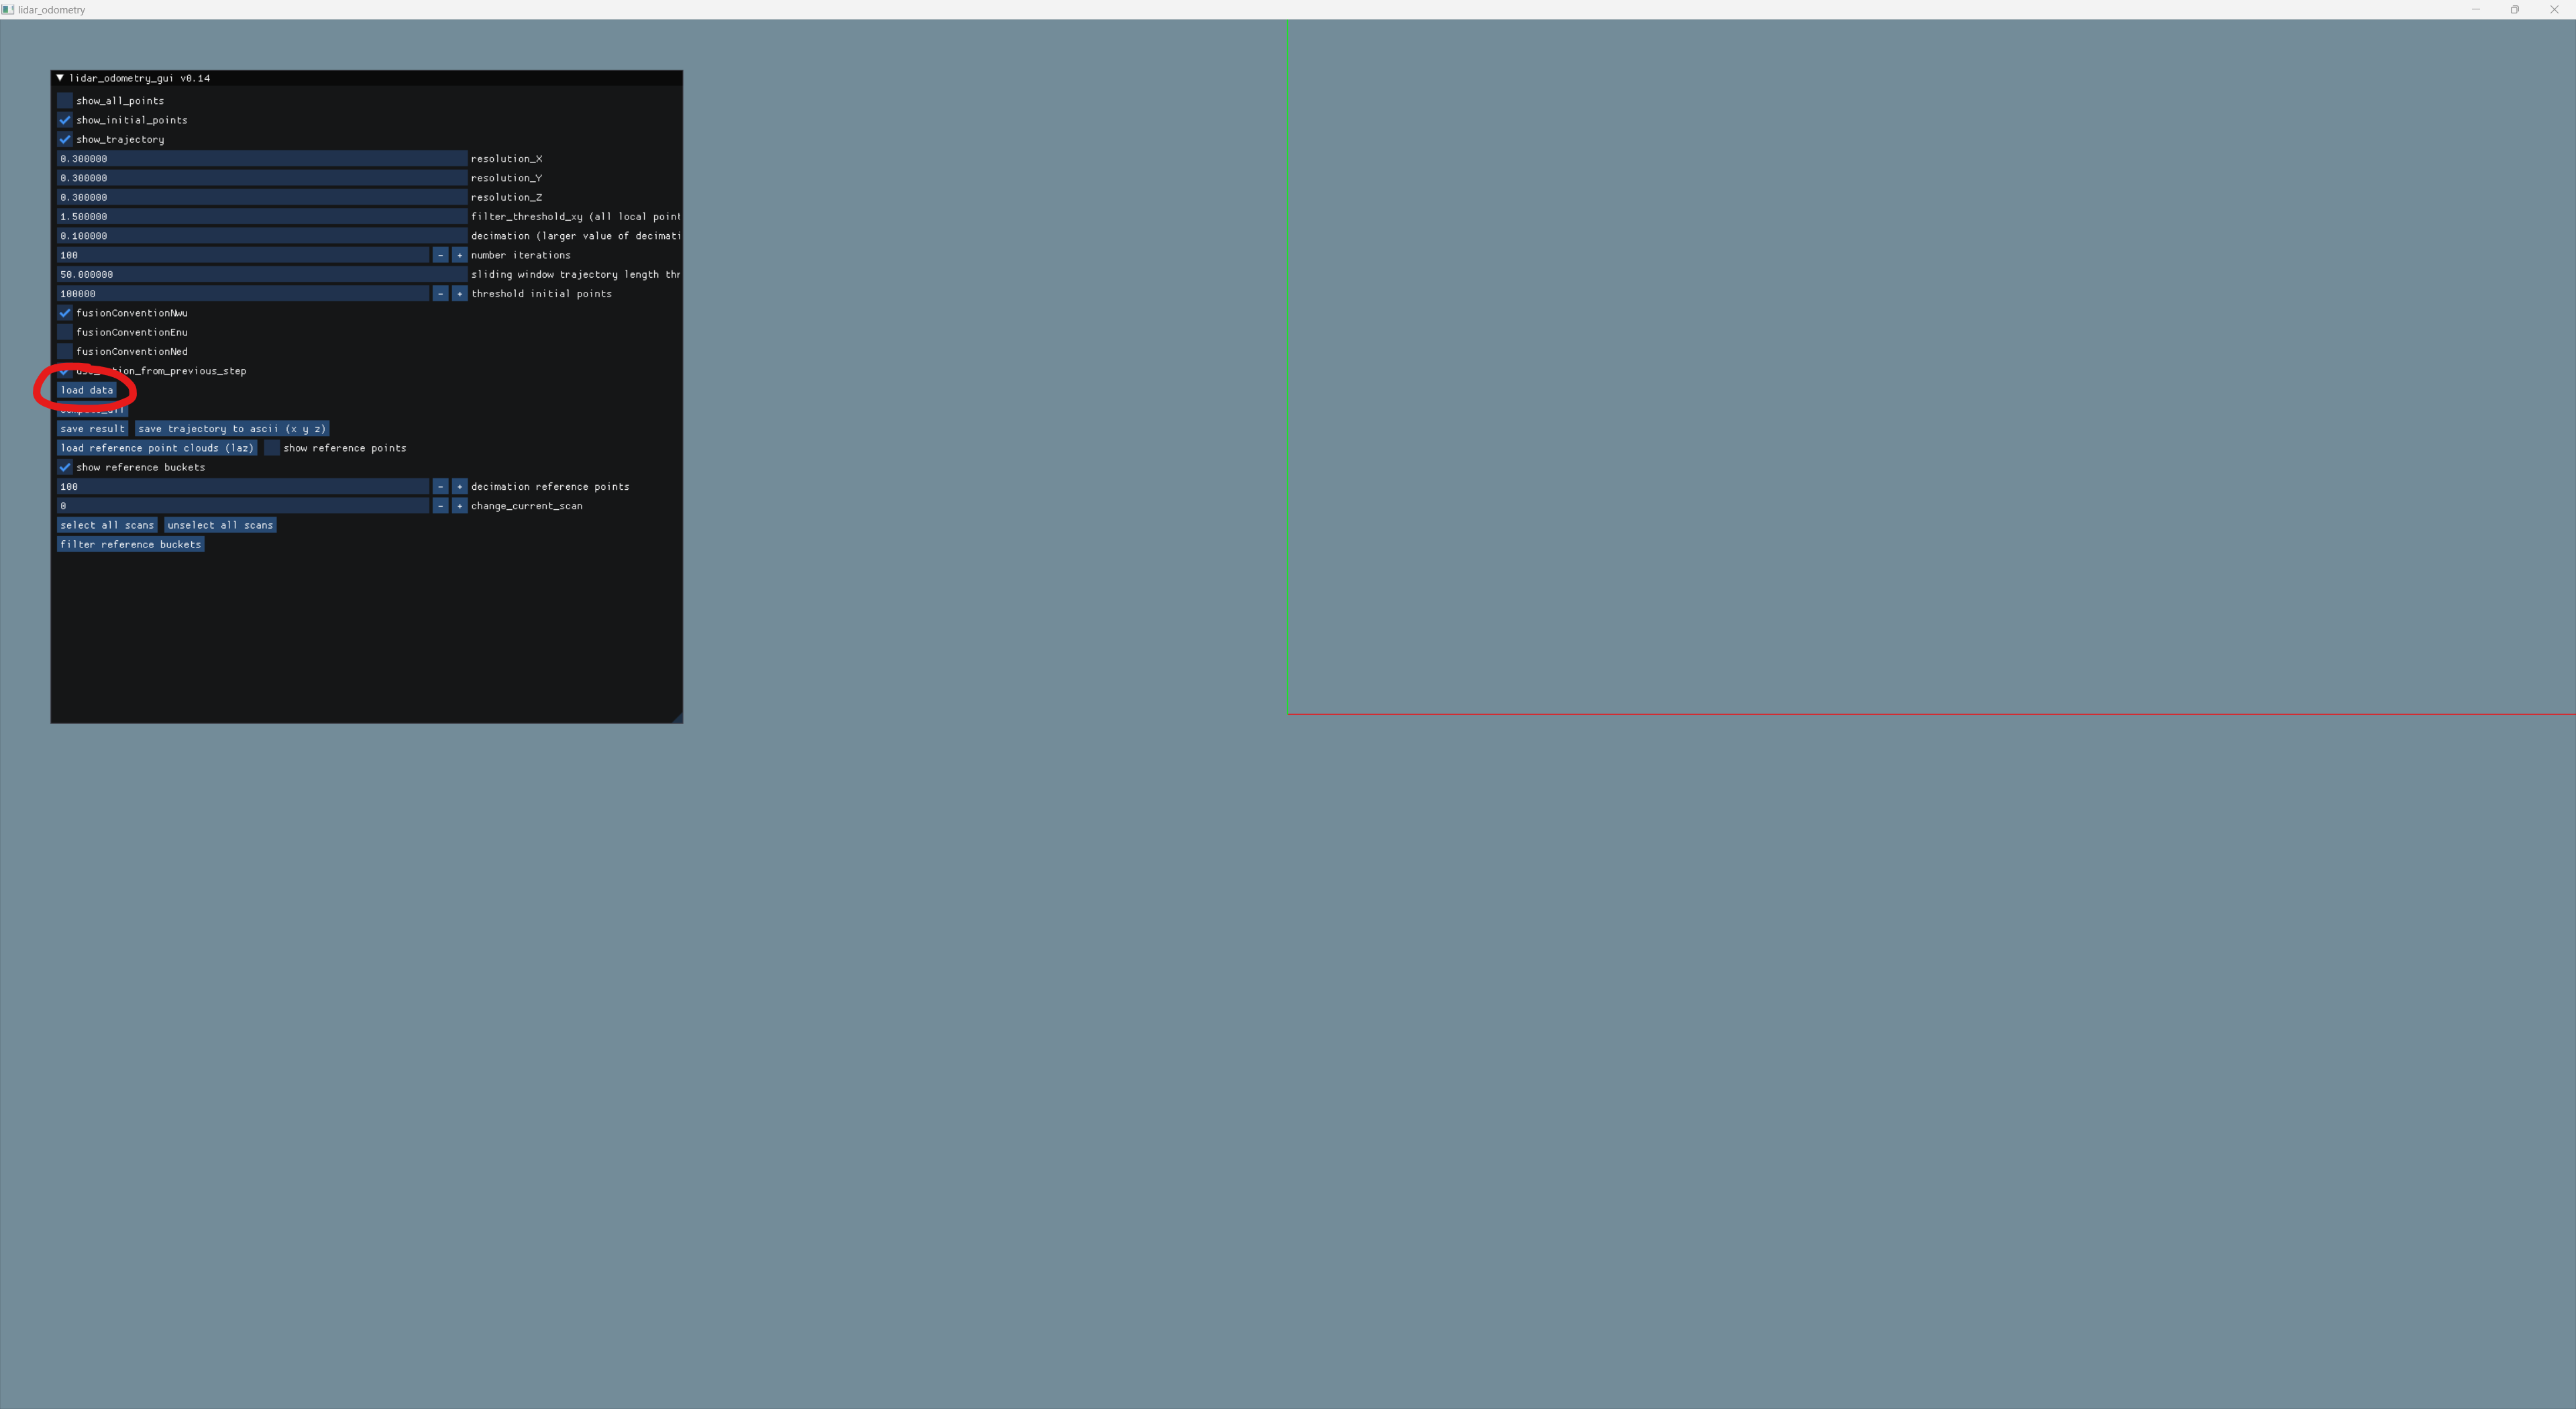
\includegraphics[width=\textwidth]{1.png}
	\caption{Step 1 - loading data.}
	\label{fig:1}
\end{figure}

\begin{figure}
	\centering
	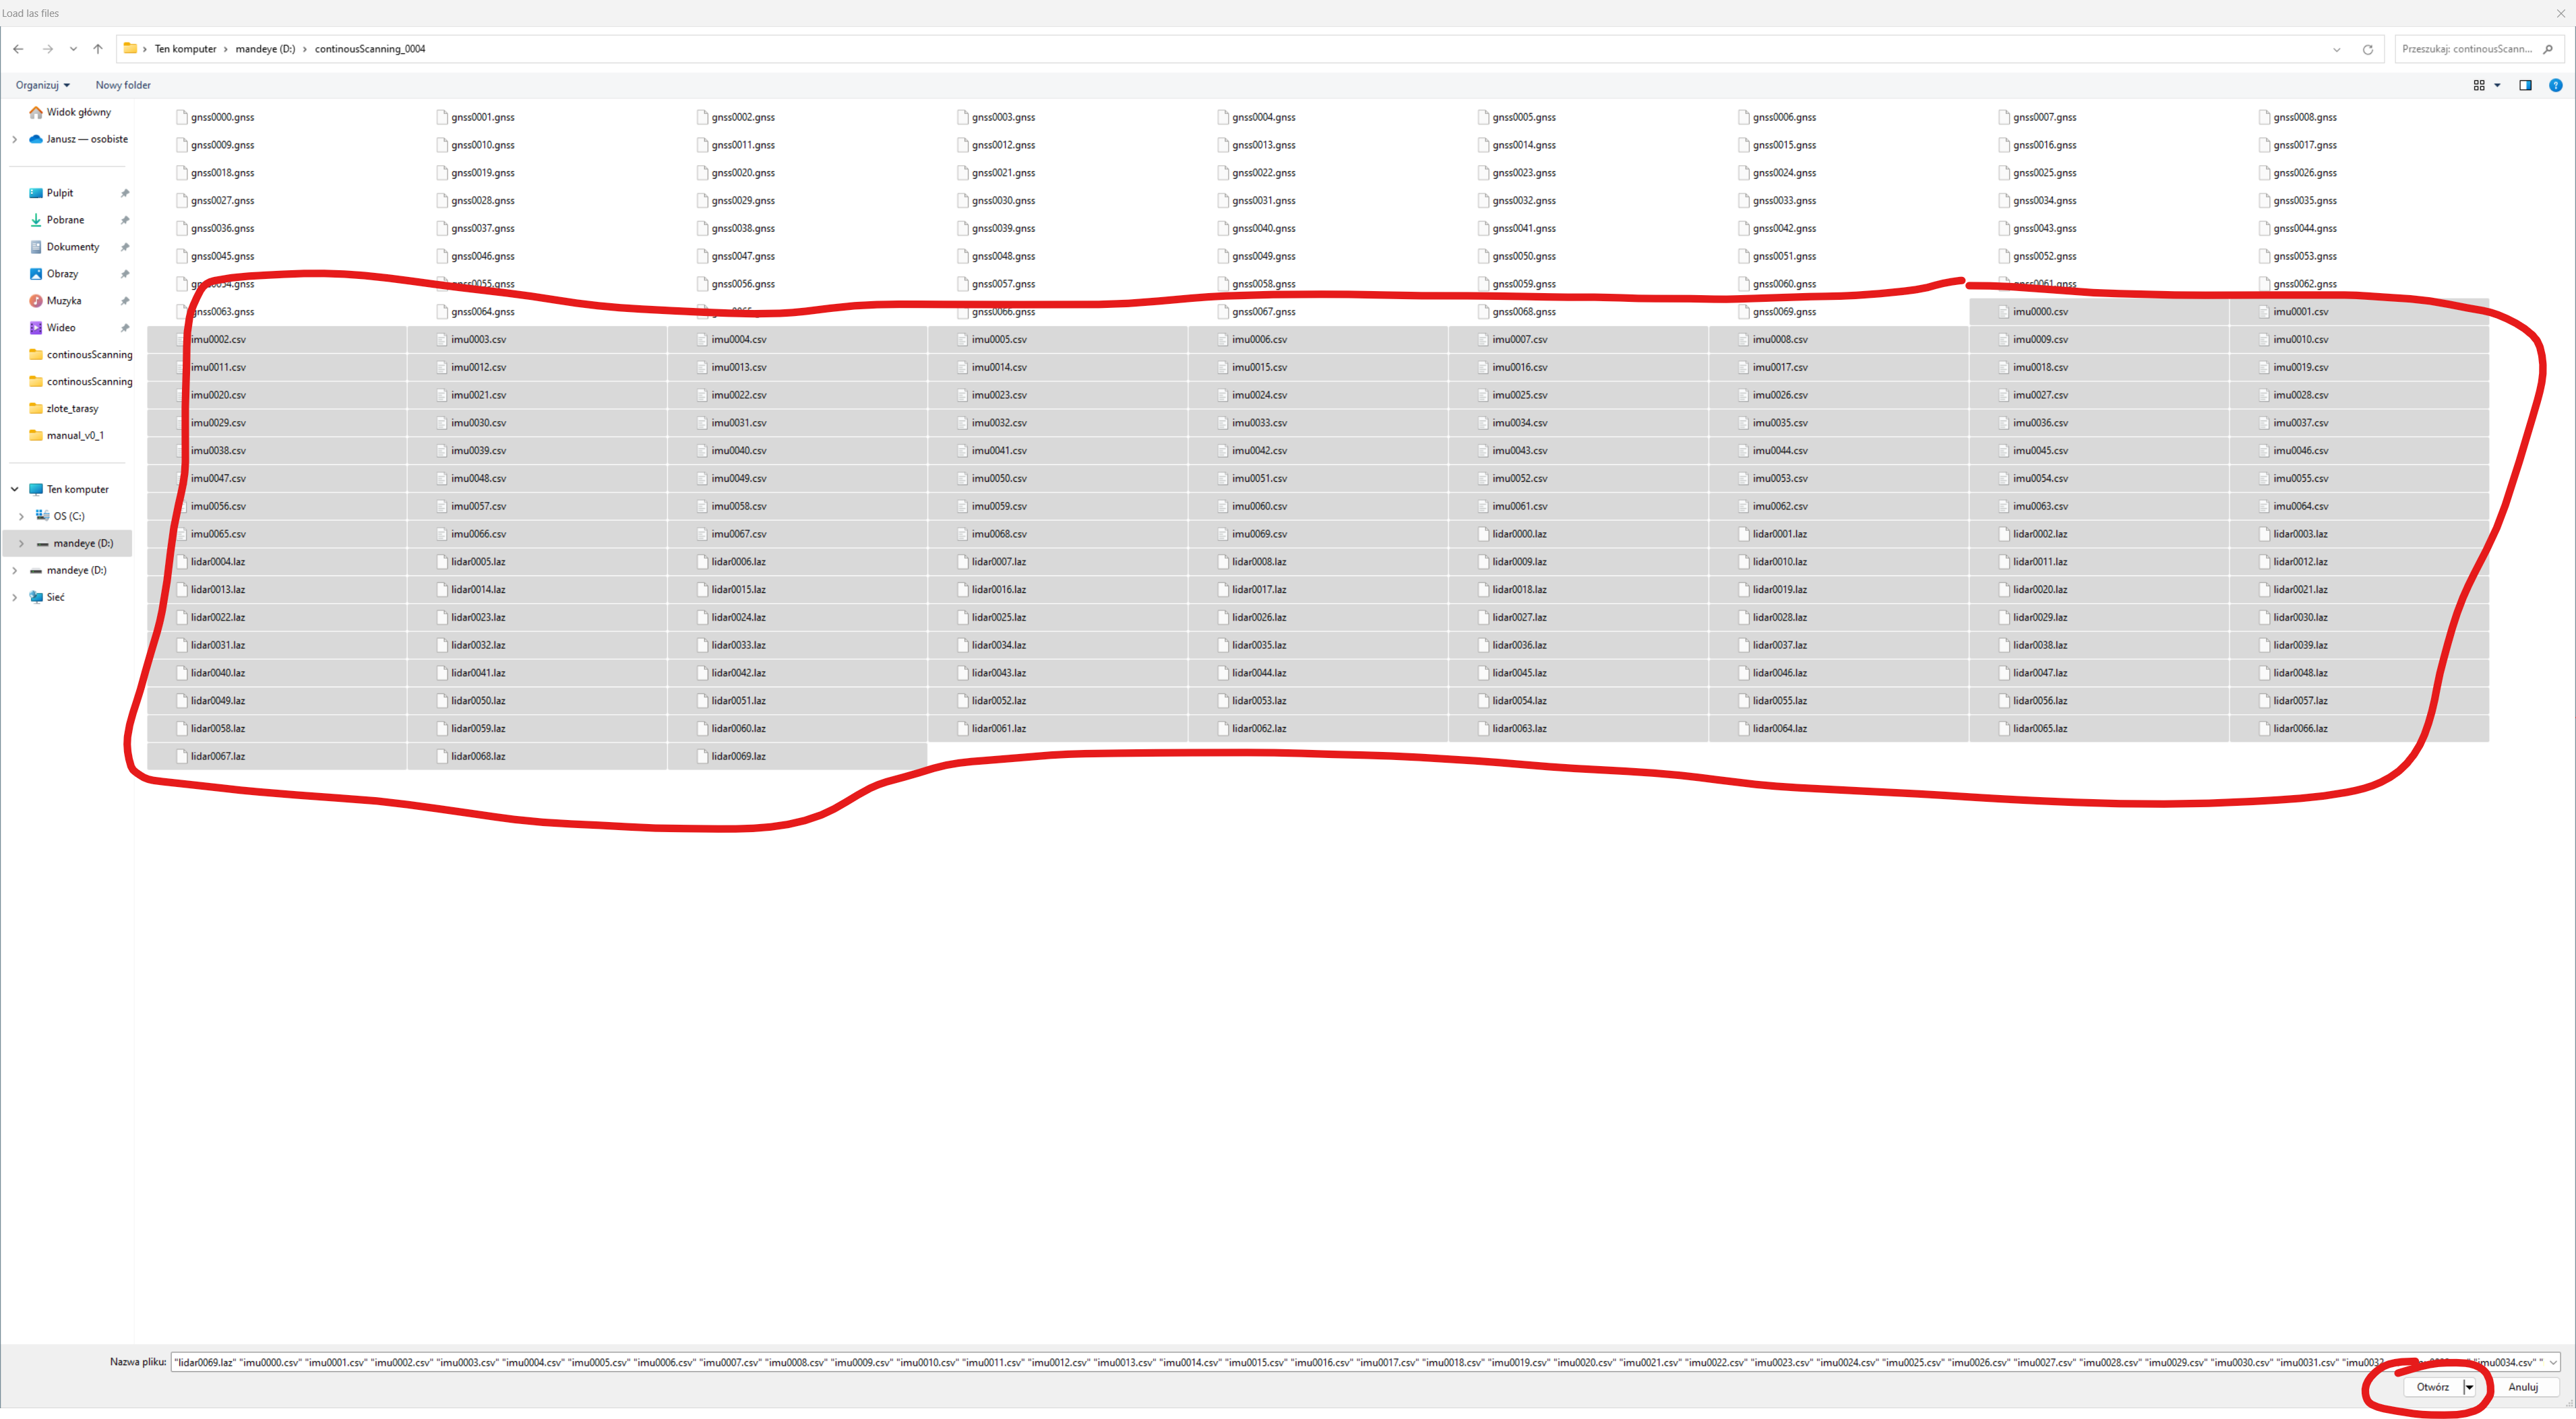
\includegraphics[width=\textwidth]{2.png}
	\caption{Step 2 - select all *.csv and *.laz files from folder that \href{https://github.com/JanuszBedkowski/mandeye_controller/blob/main/doc/manual/manual_v0_1/mandeye_dev_manual_v0_1.pdf}{MANDEYE} mobile mapping system created on USB drive.}
	\label{fig:2}
\end{figure}

\begin{figure}
	\centering
	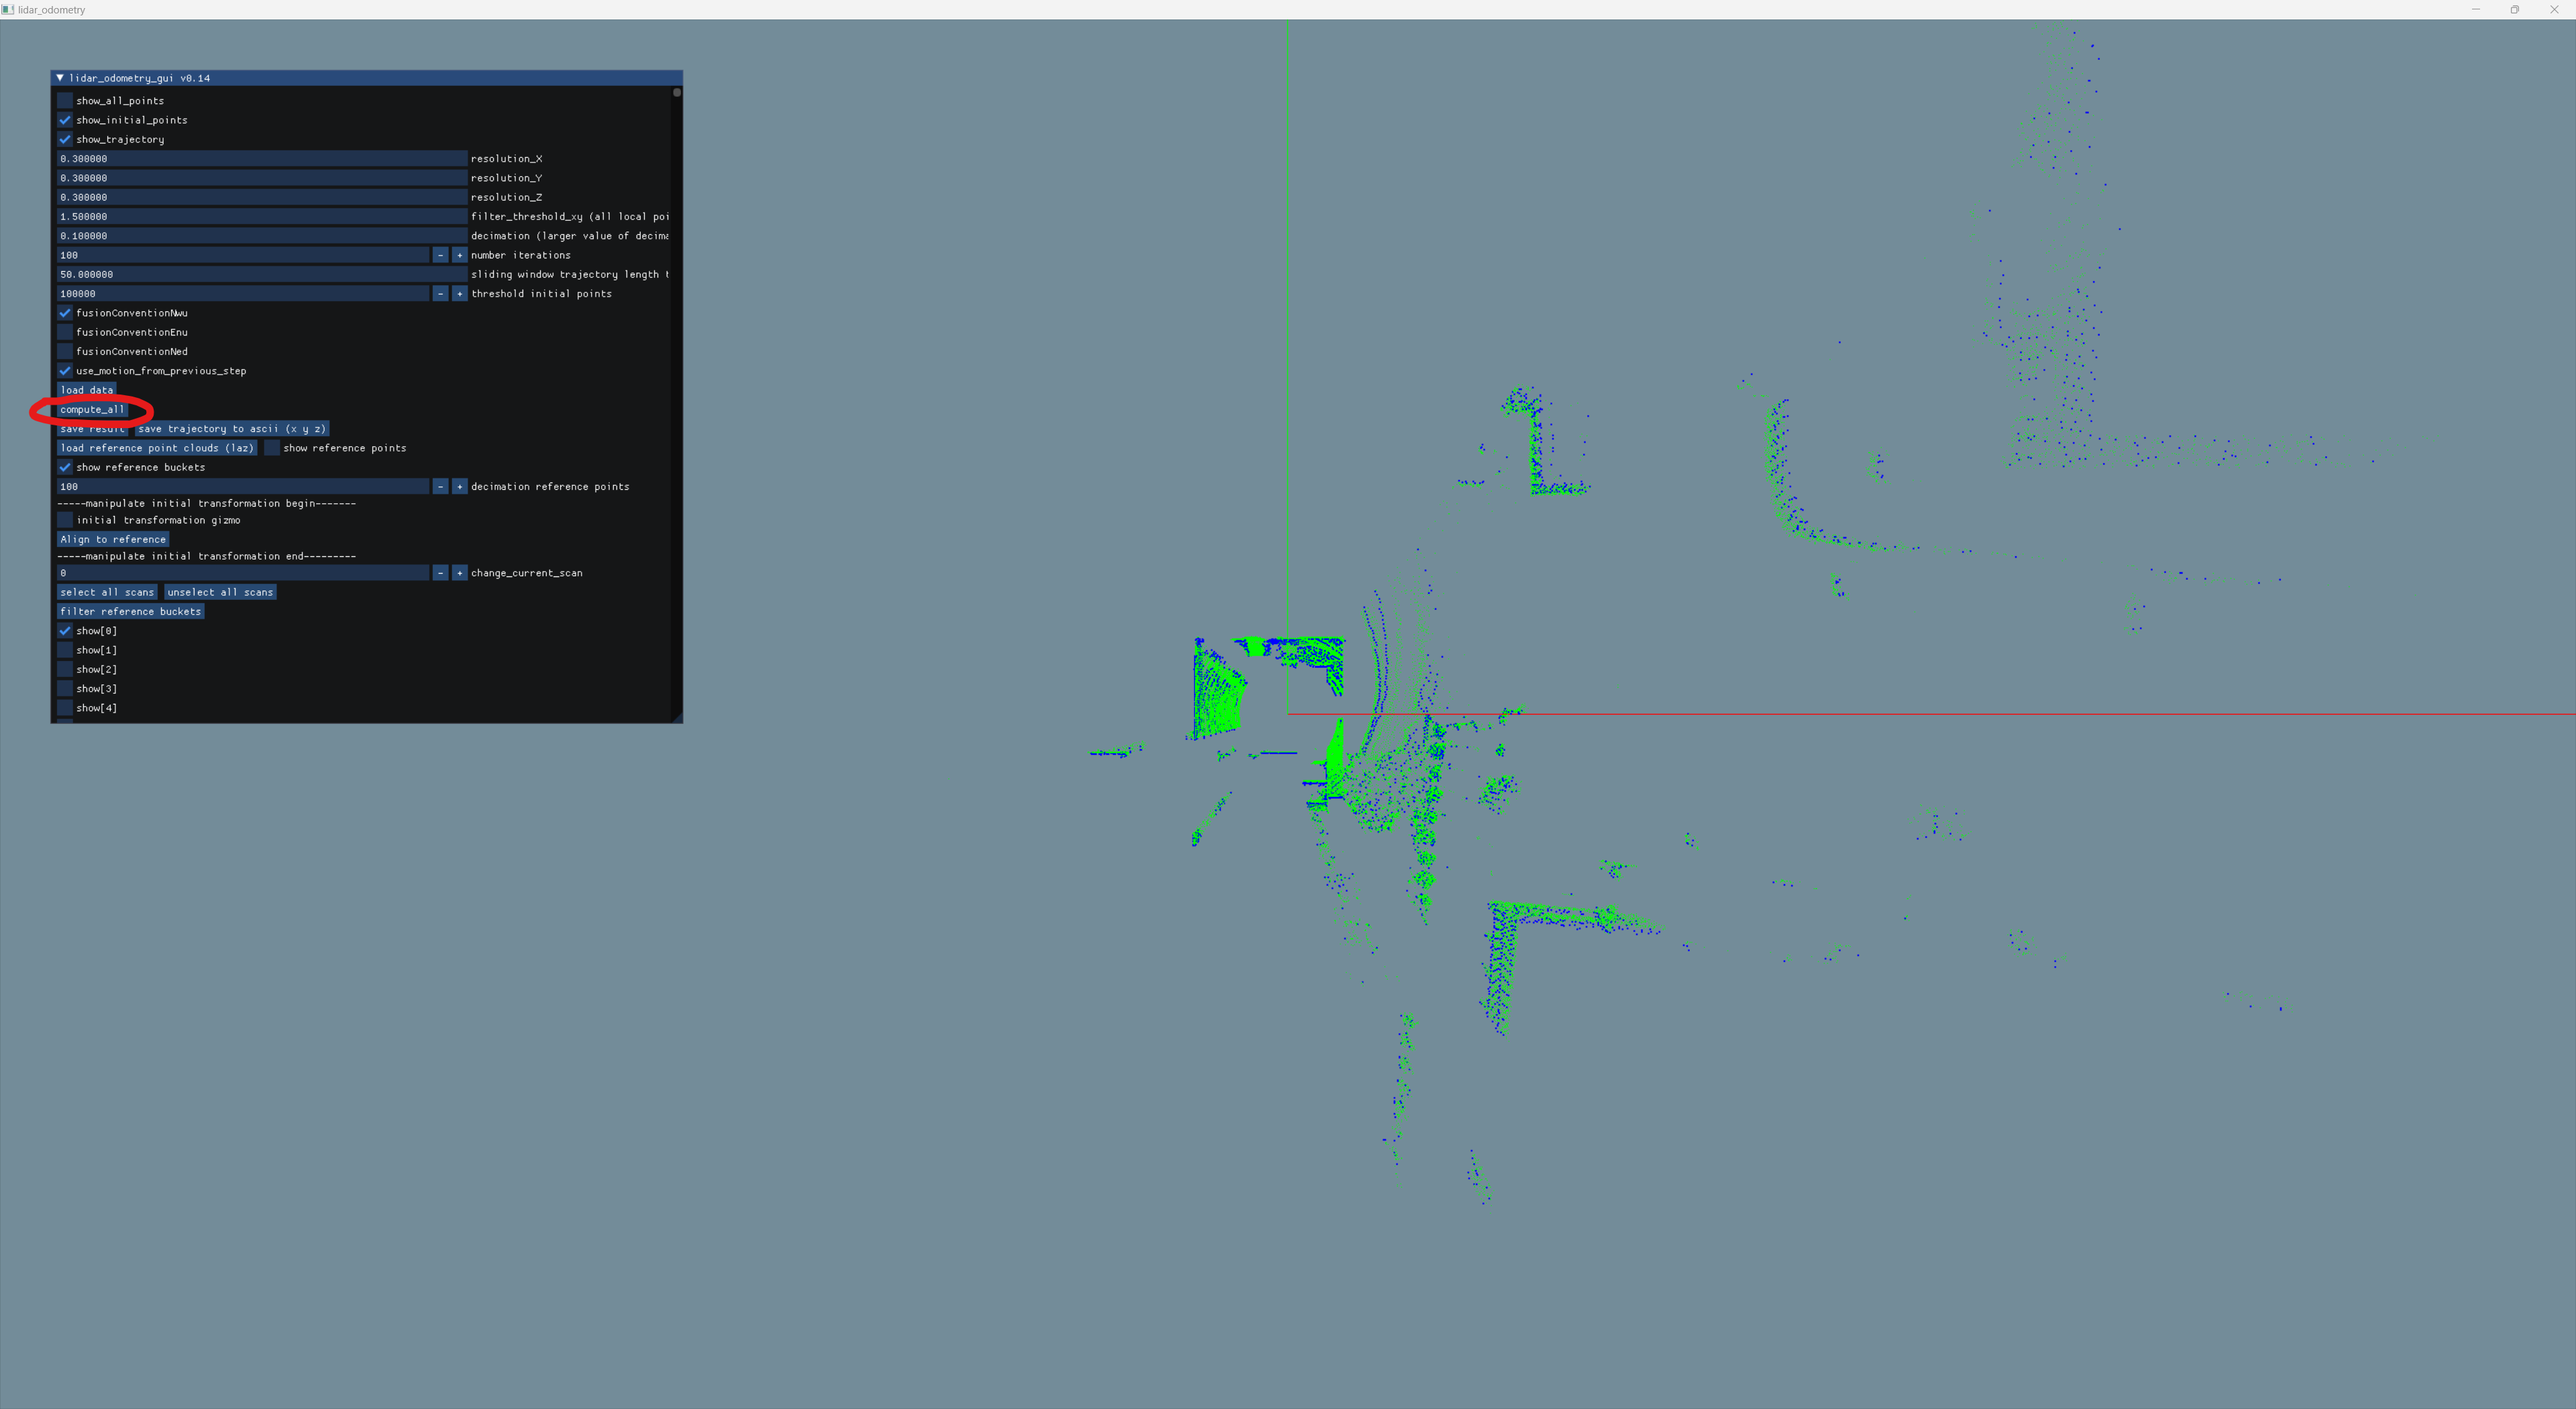
\includegraphics[width=\textwidth]{3.png}
	\caption{Step 3 - press 'compute all'. Check console mean time and folder 'preview'.}
	\label{fig:3}
\end{figure}

\begin{figure}
	\centering
	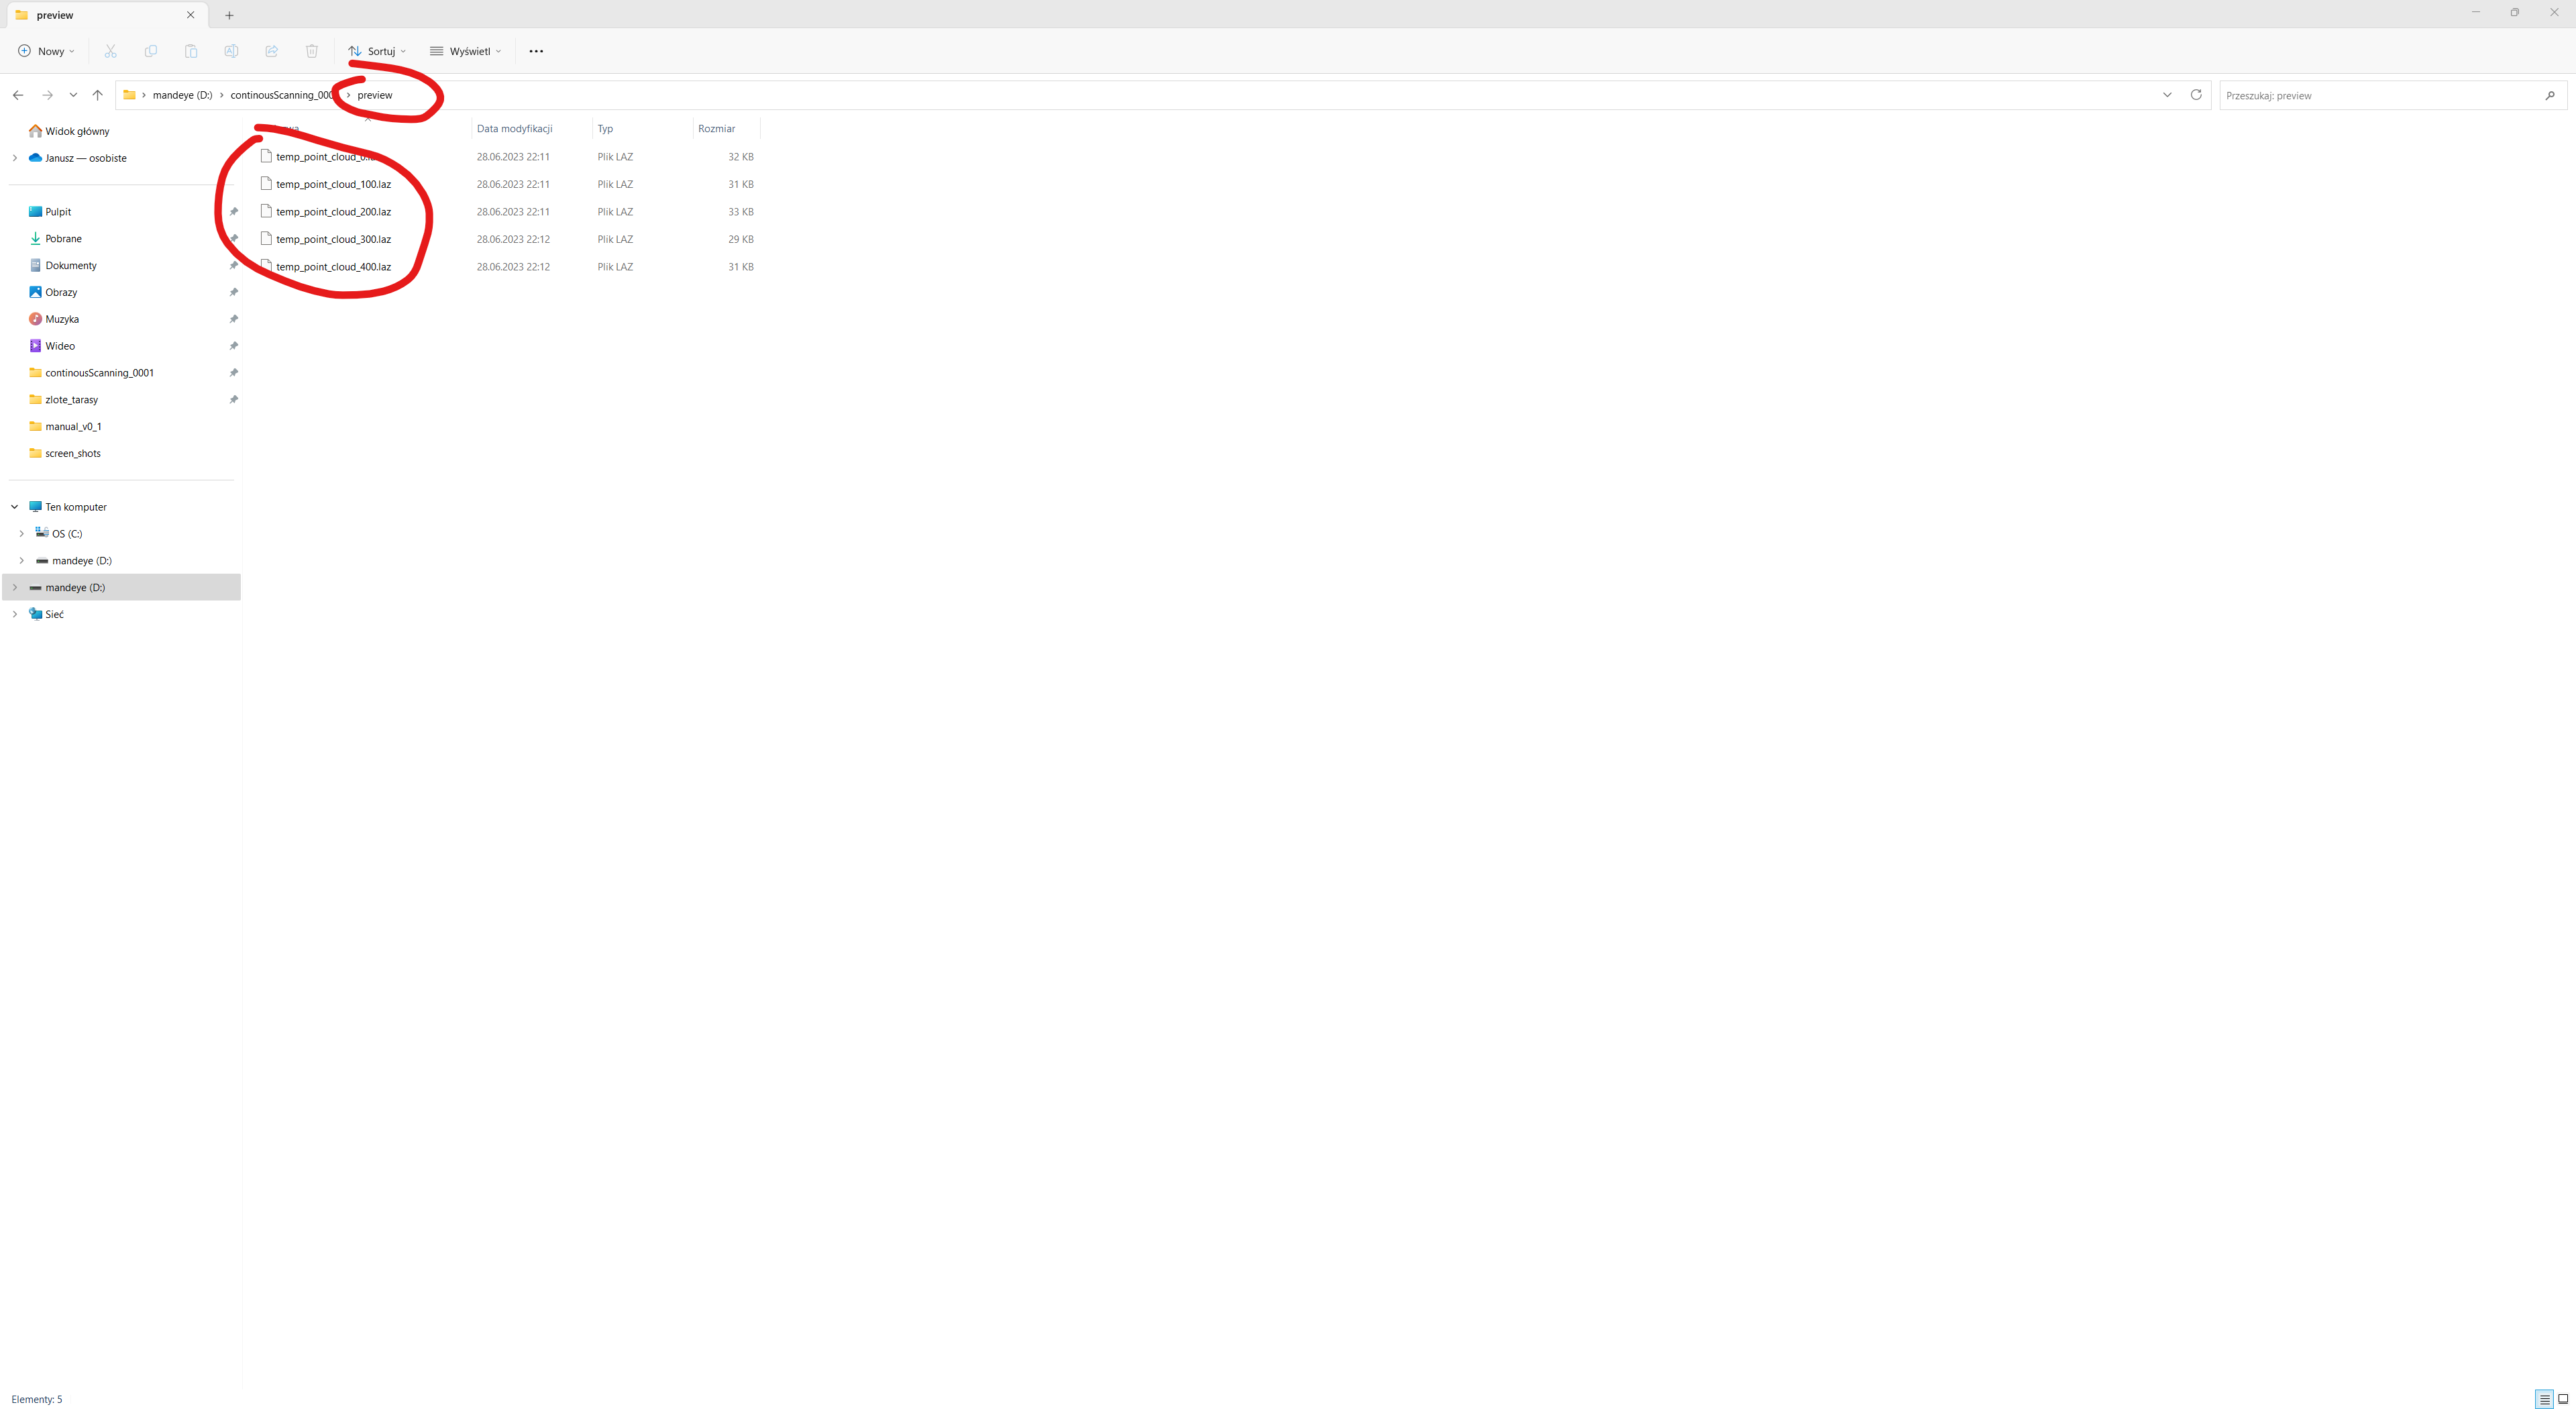
\includegraphics[width=\textwidth]{4.png}
	\caption{Optional step: intermediate results are stored in 'preview' folder.}
	\label{fig:4}
\end{figure}

\begin{figure}
	\centering
	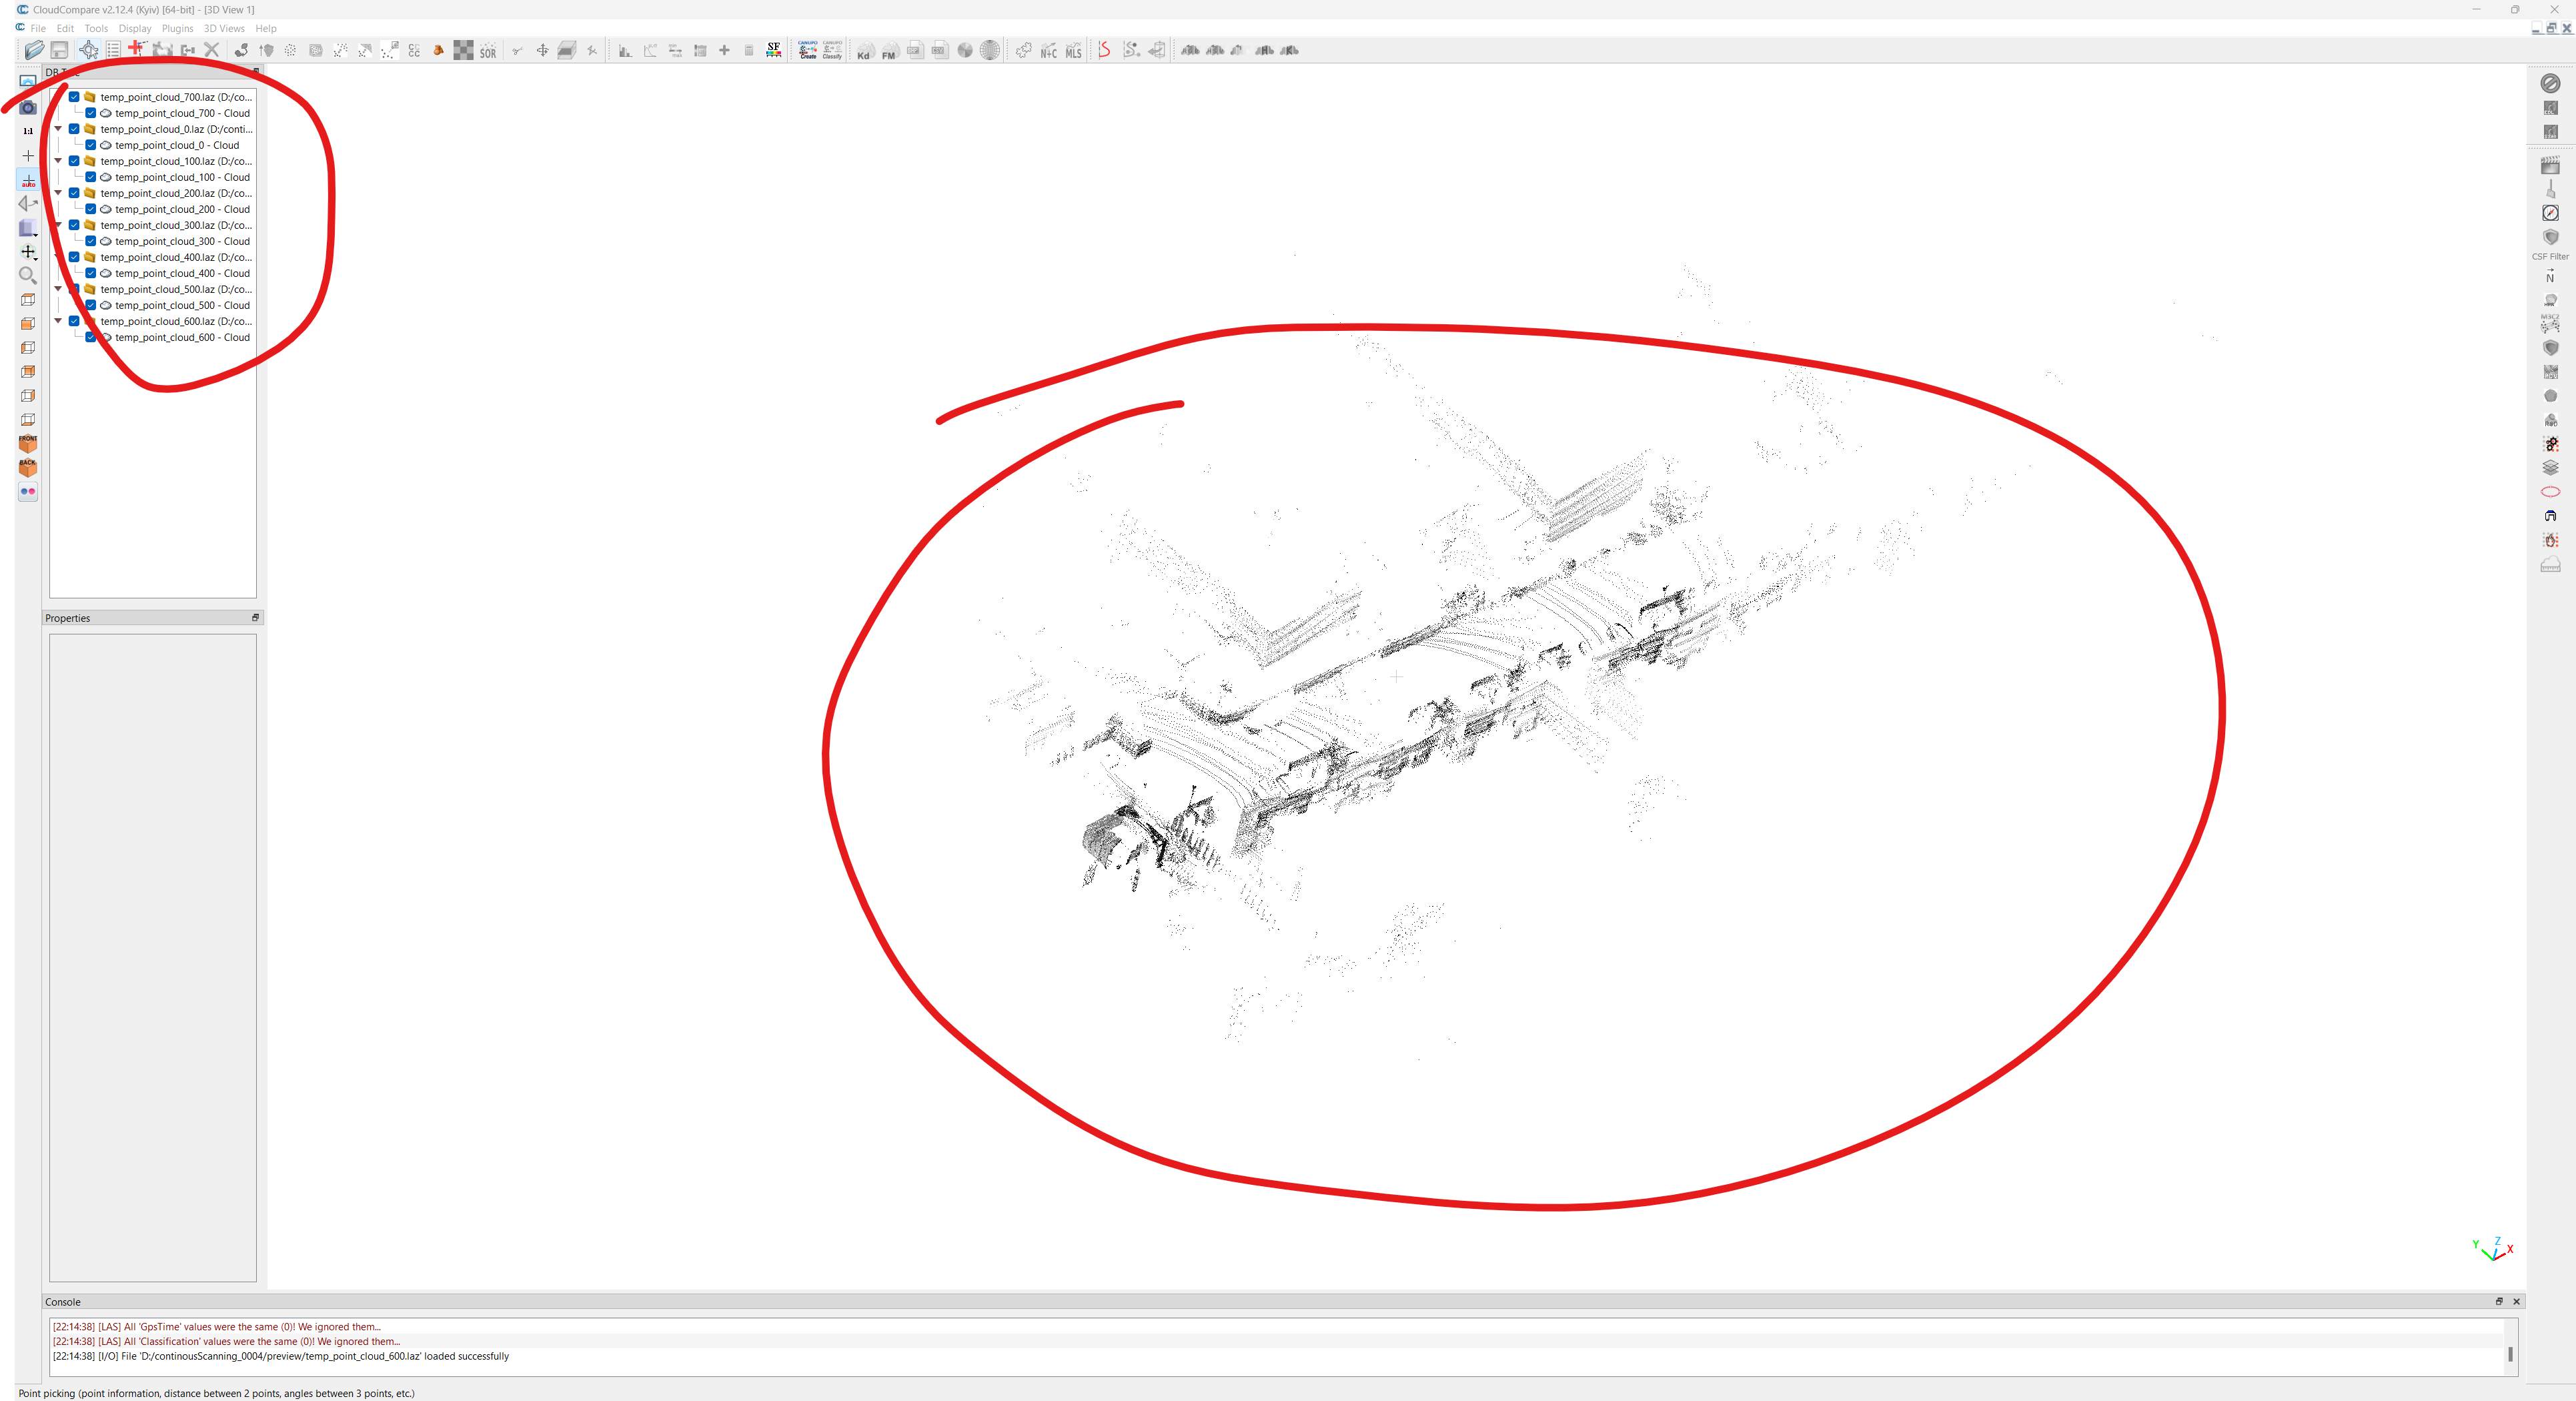
\includegraphics[width=\textwidth]{5.png}
	\caption{Optional step: You can watch the progress in open source \href{https://www.cloudcompare.org/}{CloudCompare} software by loading all *.laz files from 'preview' folder.}
	\label{fig:5}
\end{figure}

\begin{figure}
	\centering
	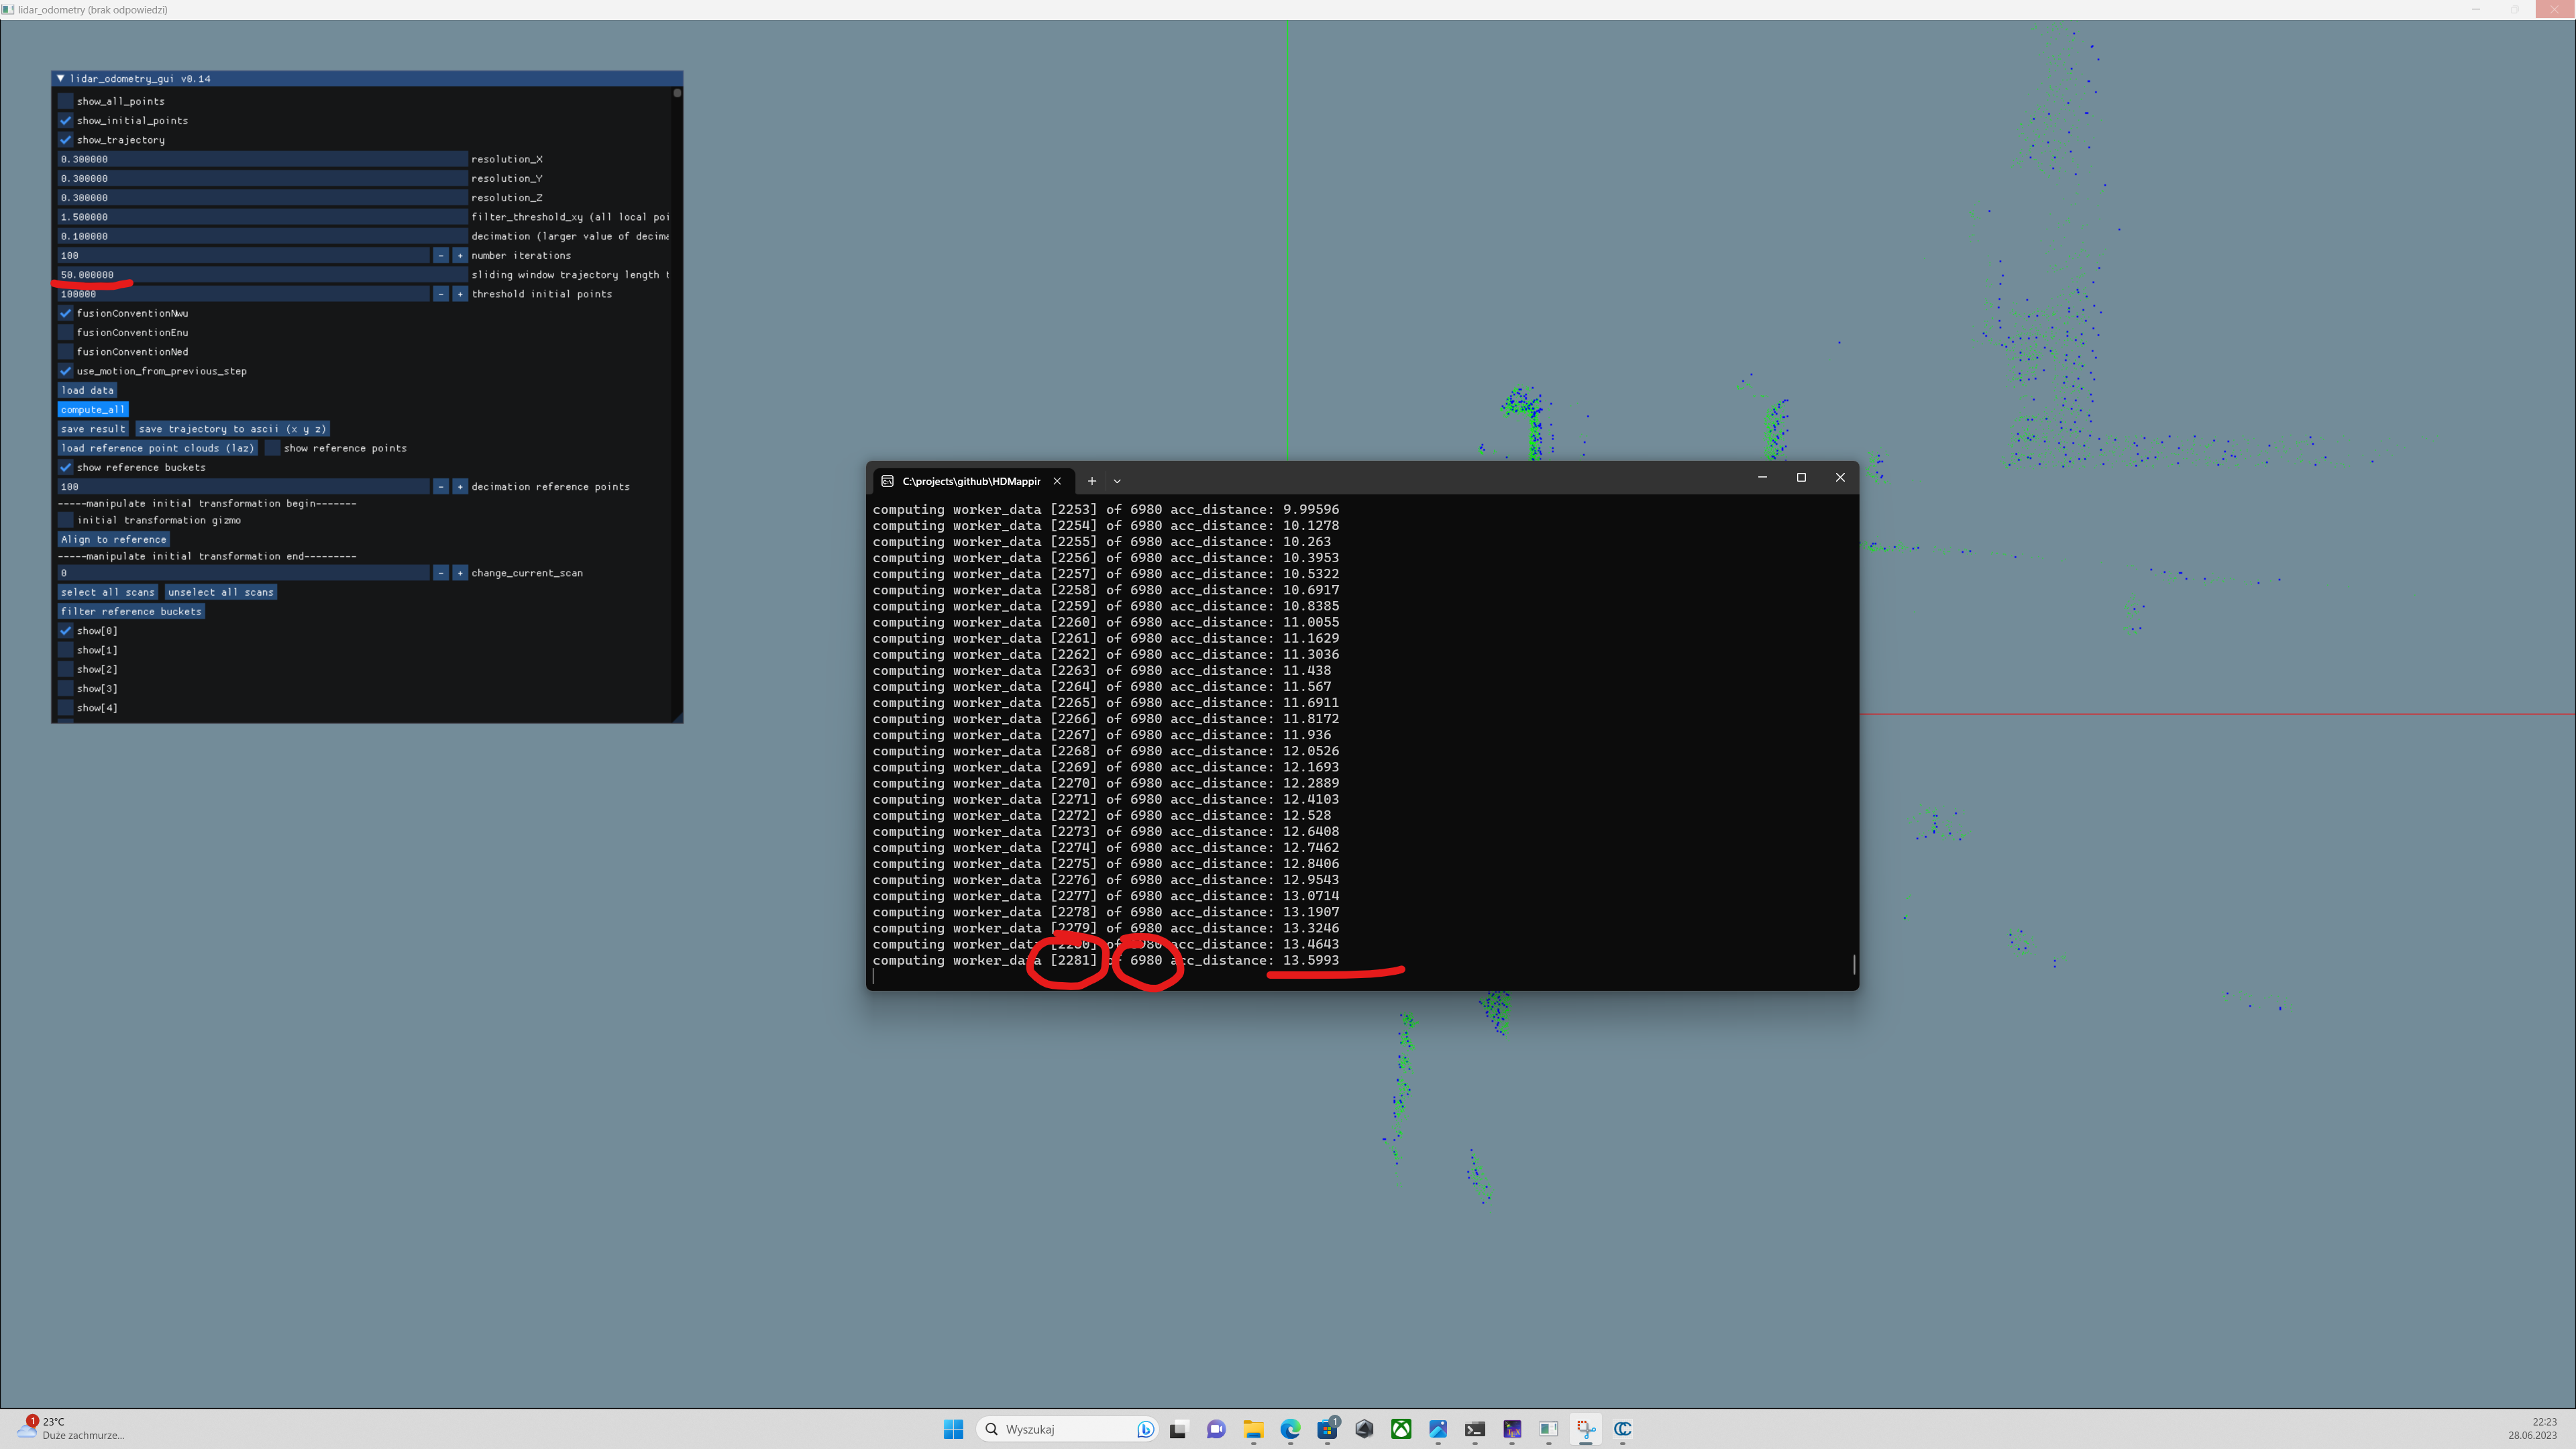
\includegraphics[width=\textwidth]{6.png}
	\caption{Progress in console.}
	\label{fig:6}
\end{figure}

\begin{figure}
	\centering
	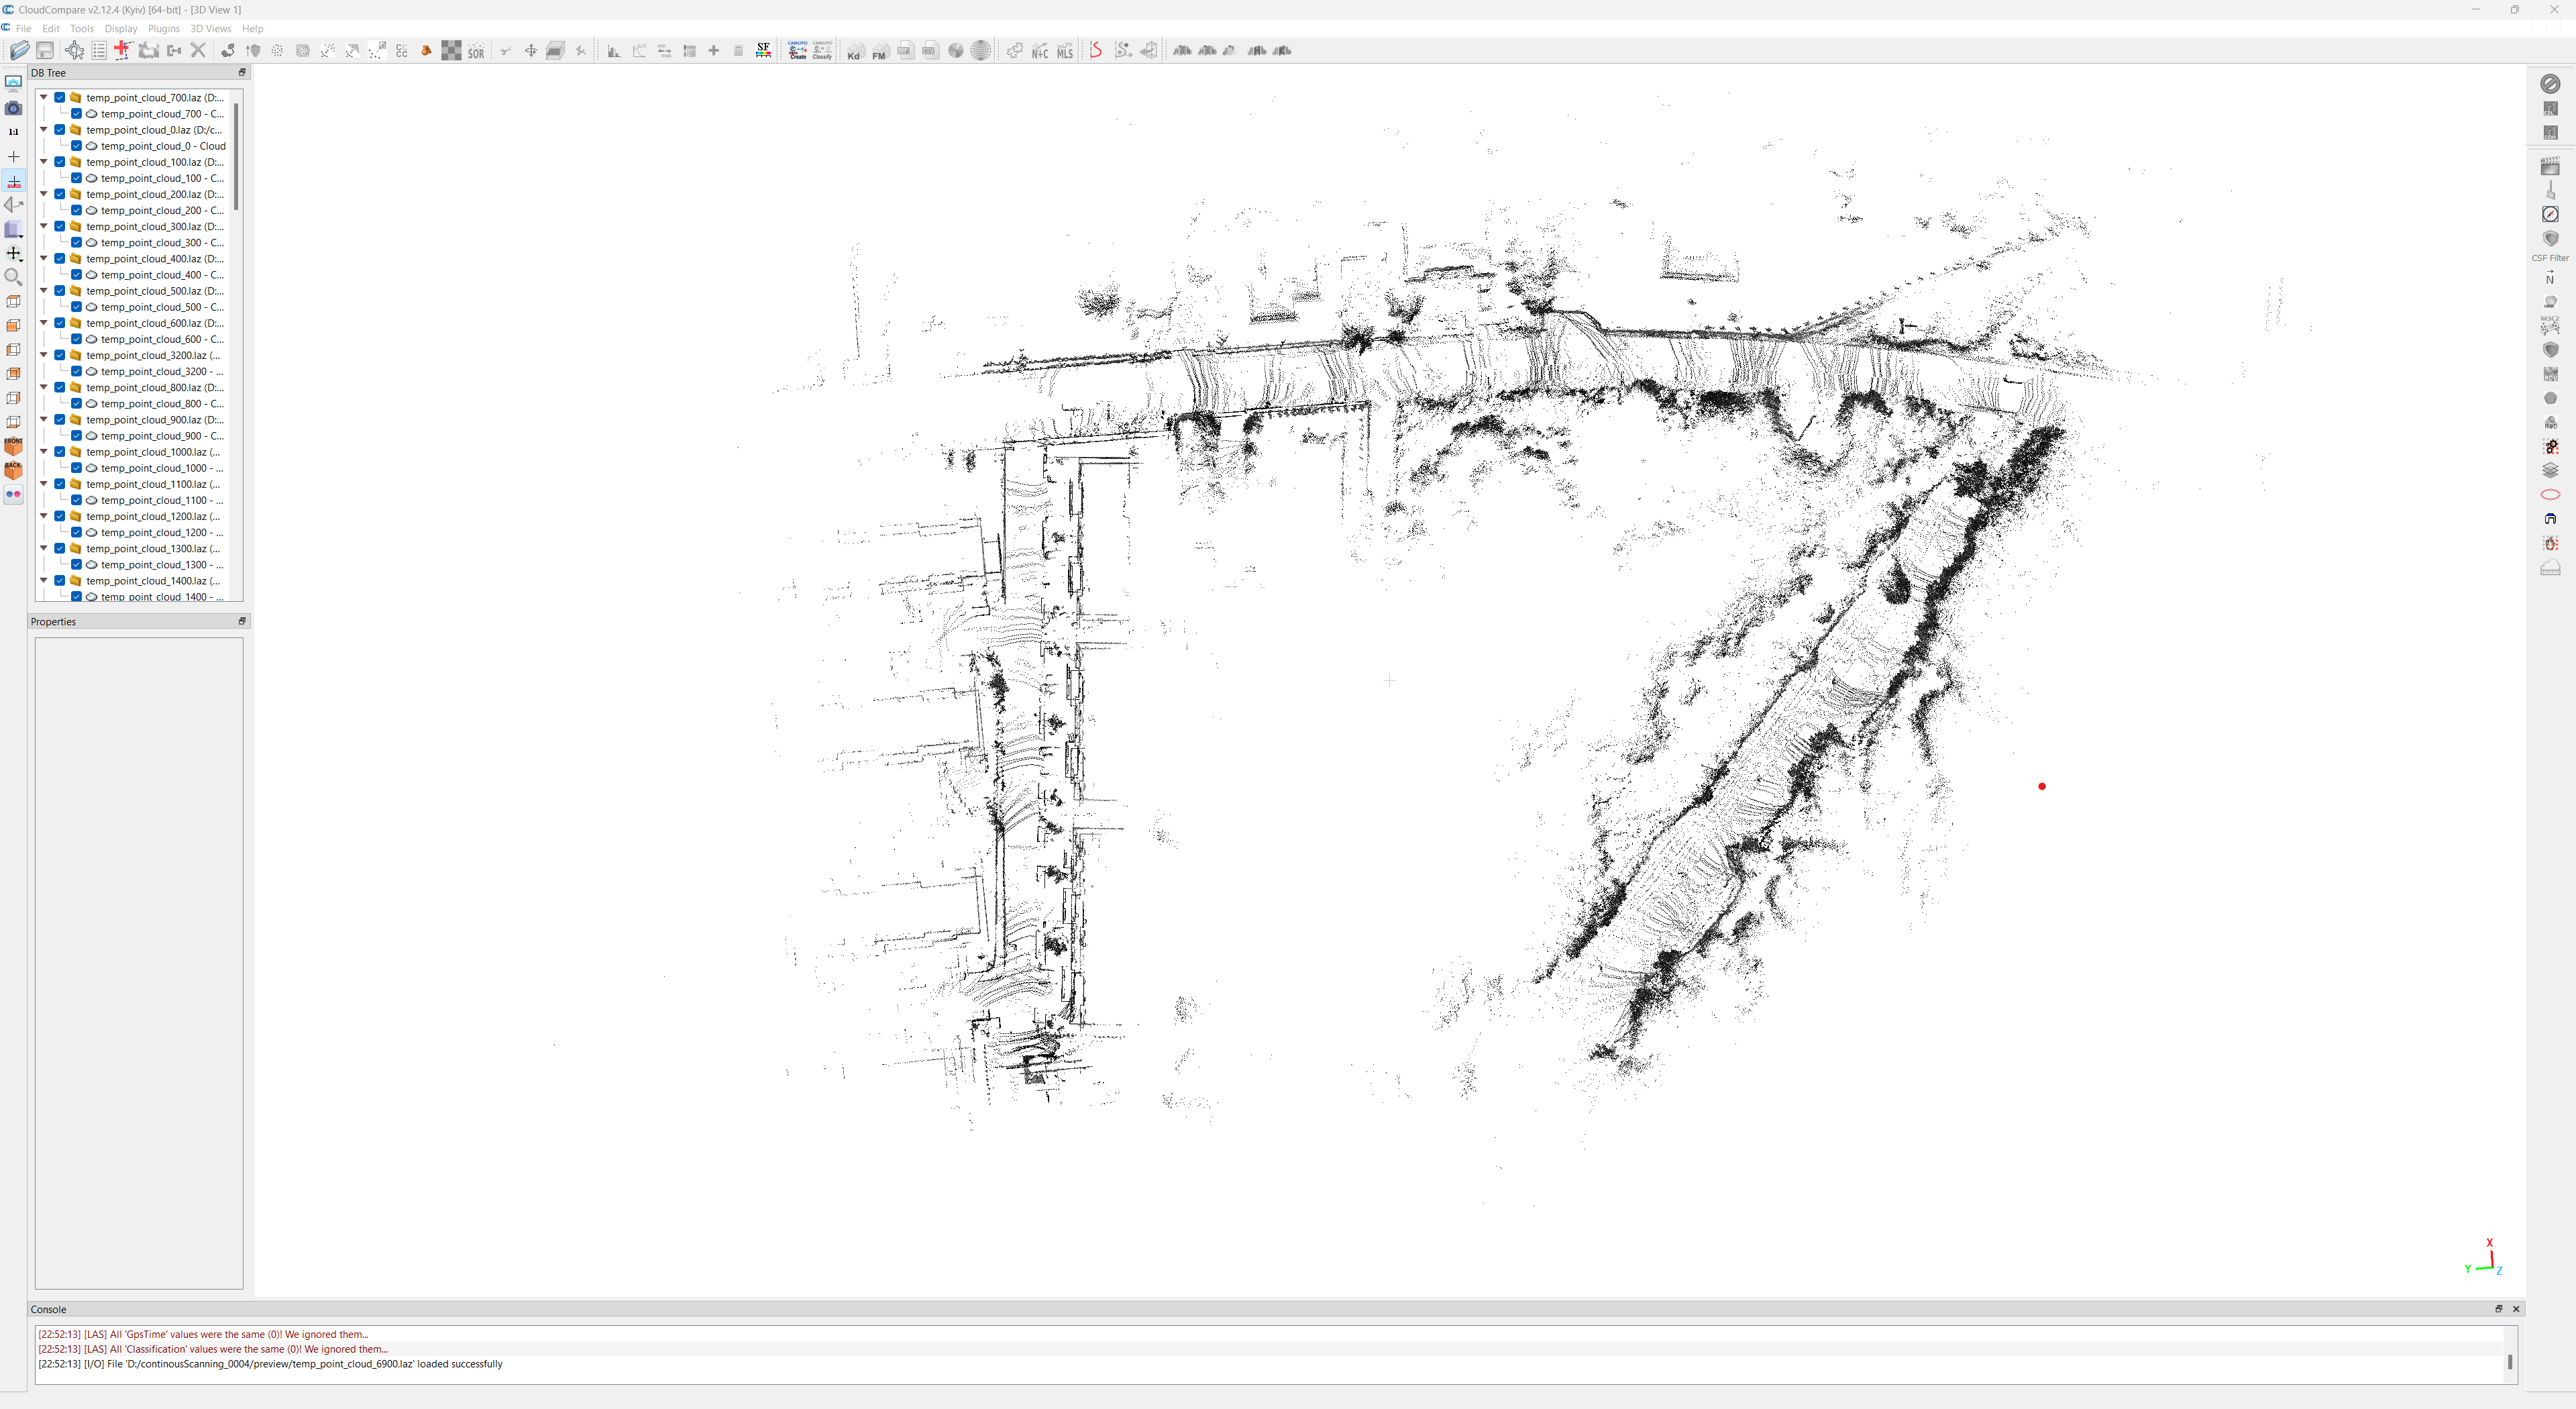
\includegraphics[width=\textwidth]{7.png}
	\caption{Final data in \href{https://www.cloudcompare.org/}{CloudCompare}.}
	\label{fig:7}
\end{figure}

\begin{figure}
	\centering
	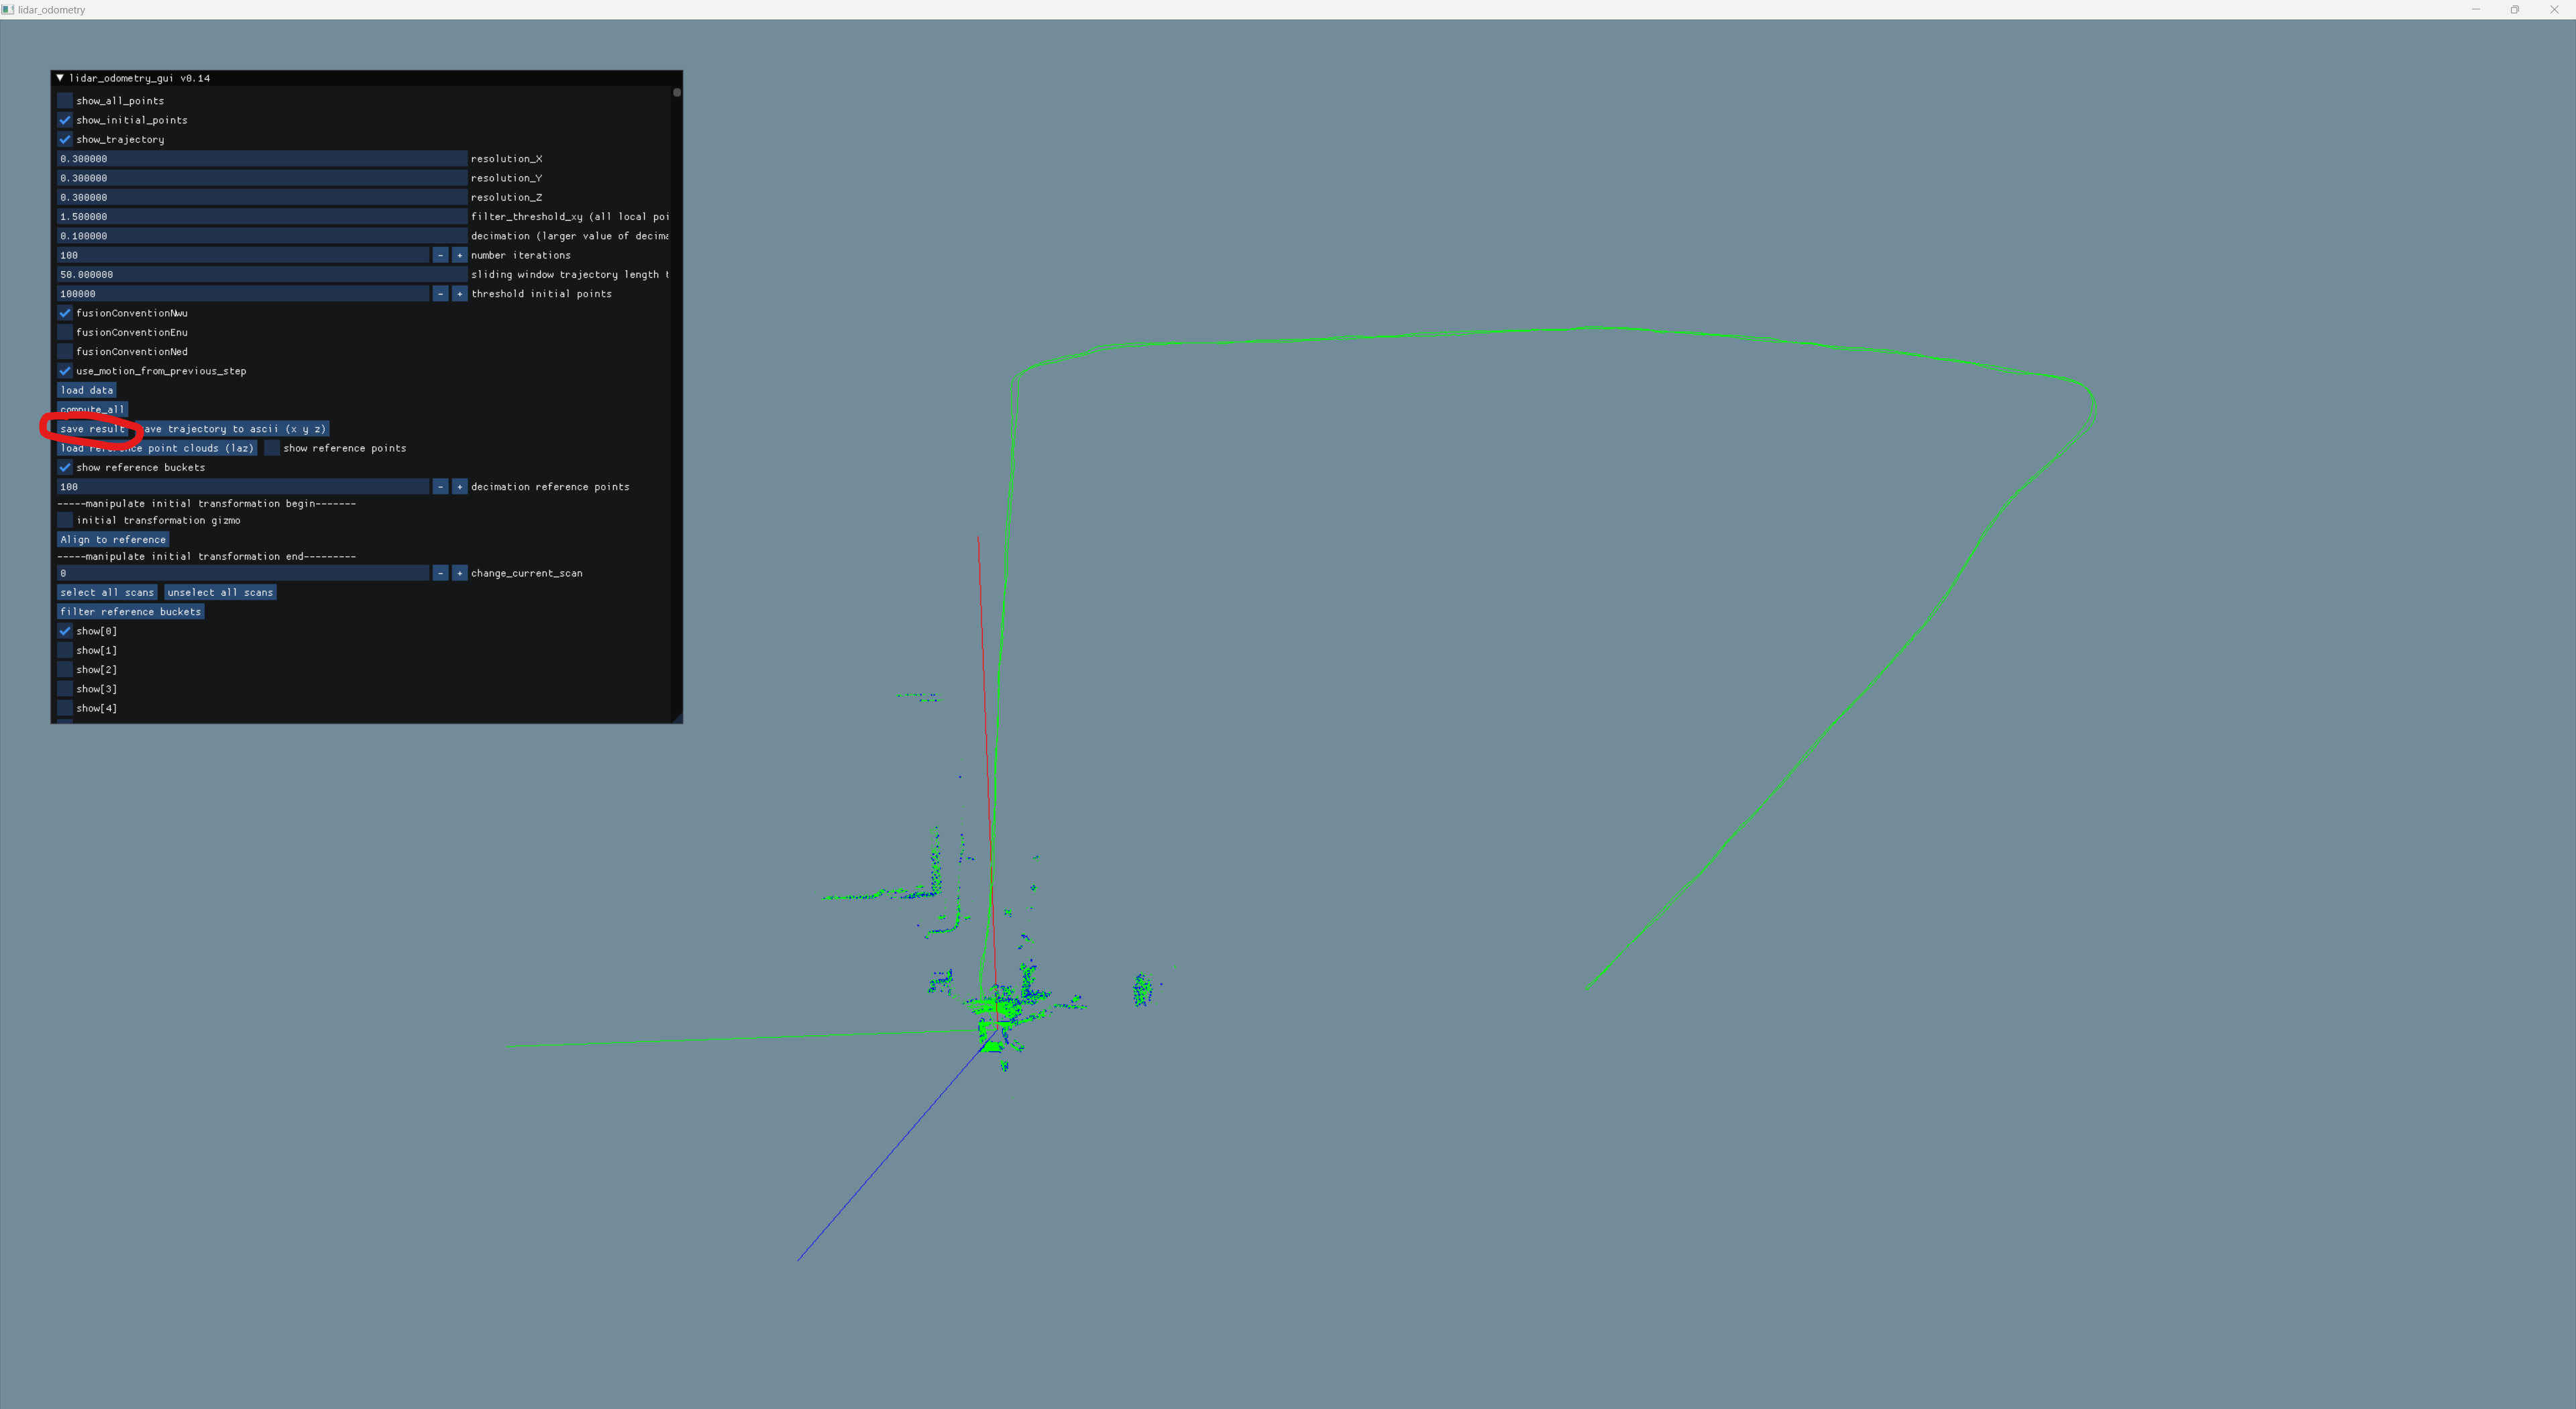
\includegraphics[width=\textwidth]{8.png}
	\caption{Final data ready for export.}
	\label{fig:8}
\end{figure}

\begin{figure}
	\centering
	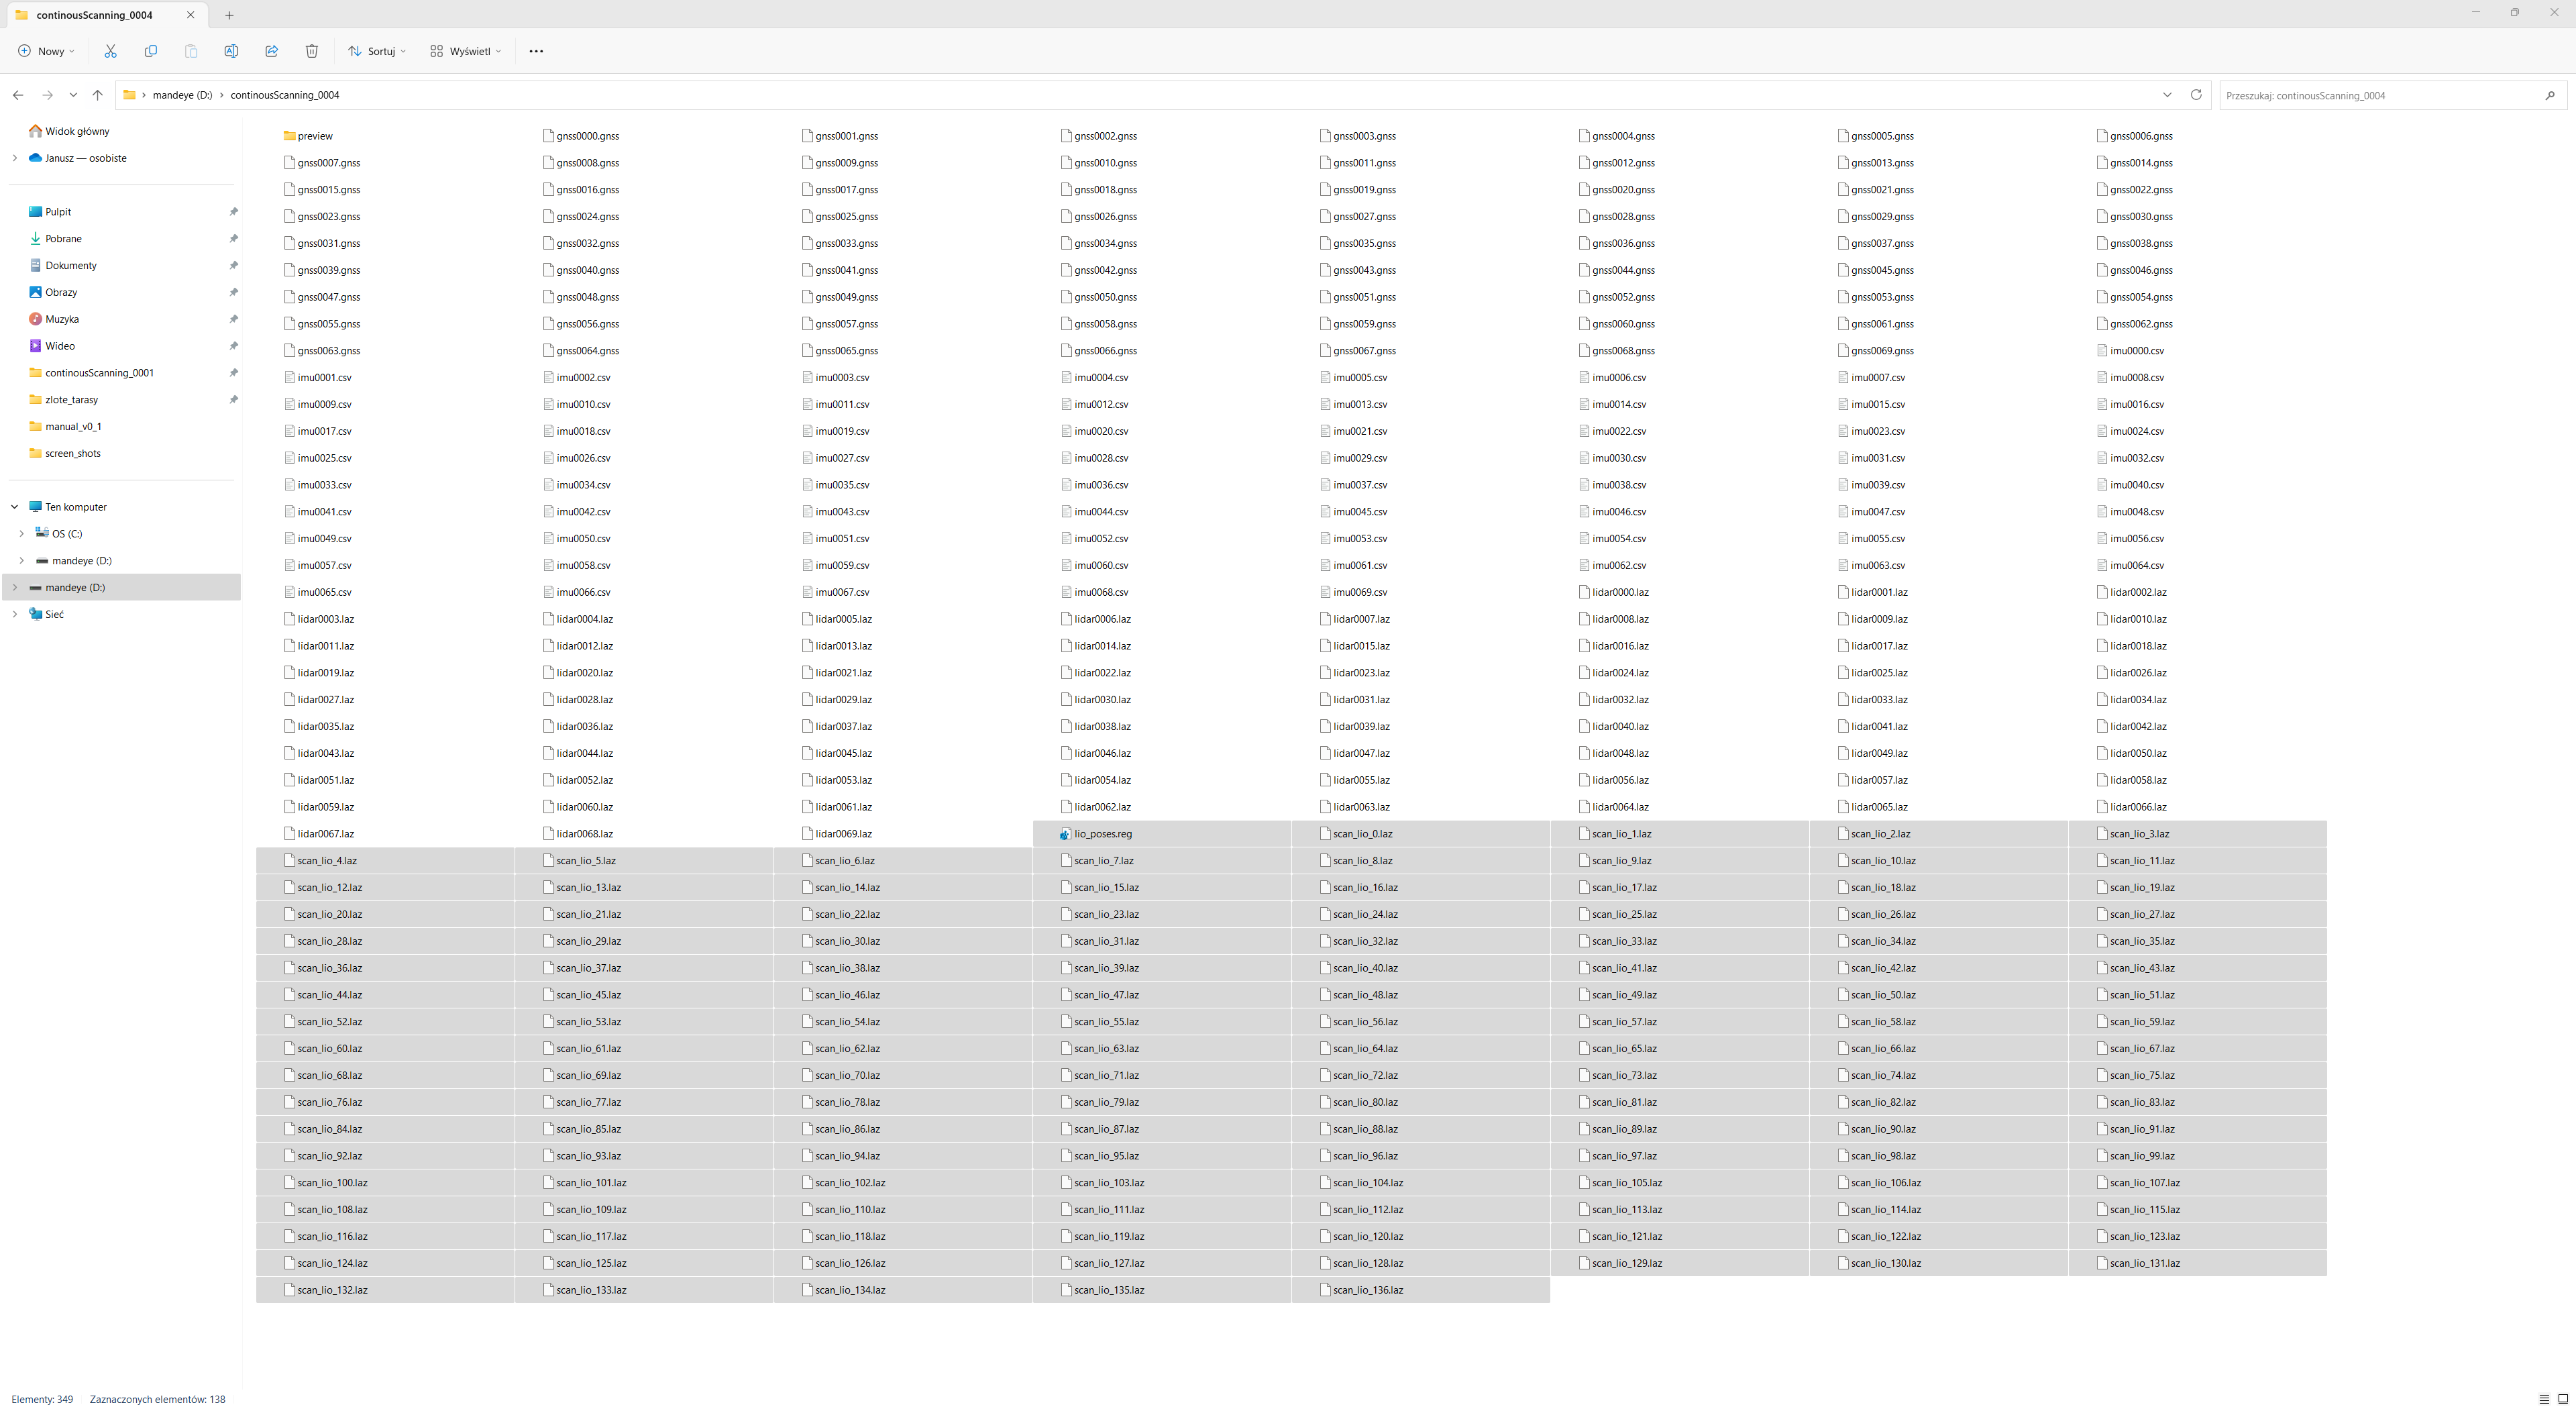
\includegraphics[width=\textwidth]{9.png}
	\caption{Exported final files.}
	\label{fig:9}
\end{figure}

\chapter{Multi view terrestrial laser scan registration}

\begin{figure}
	\centering
	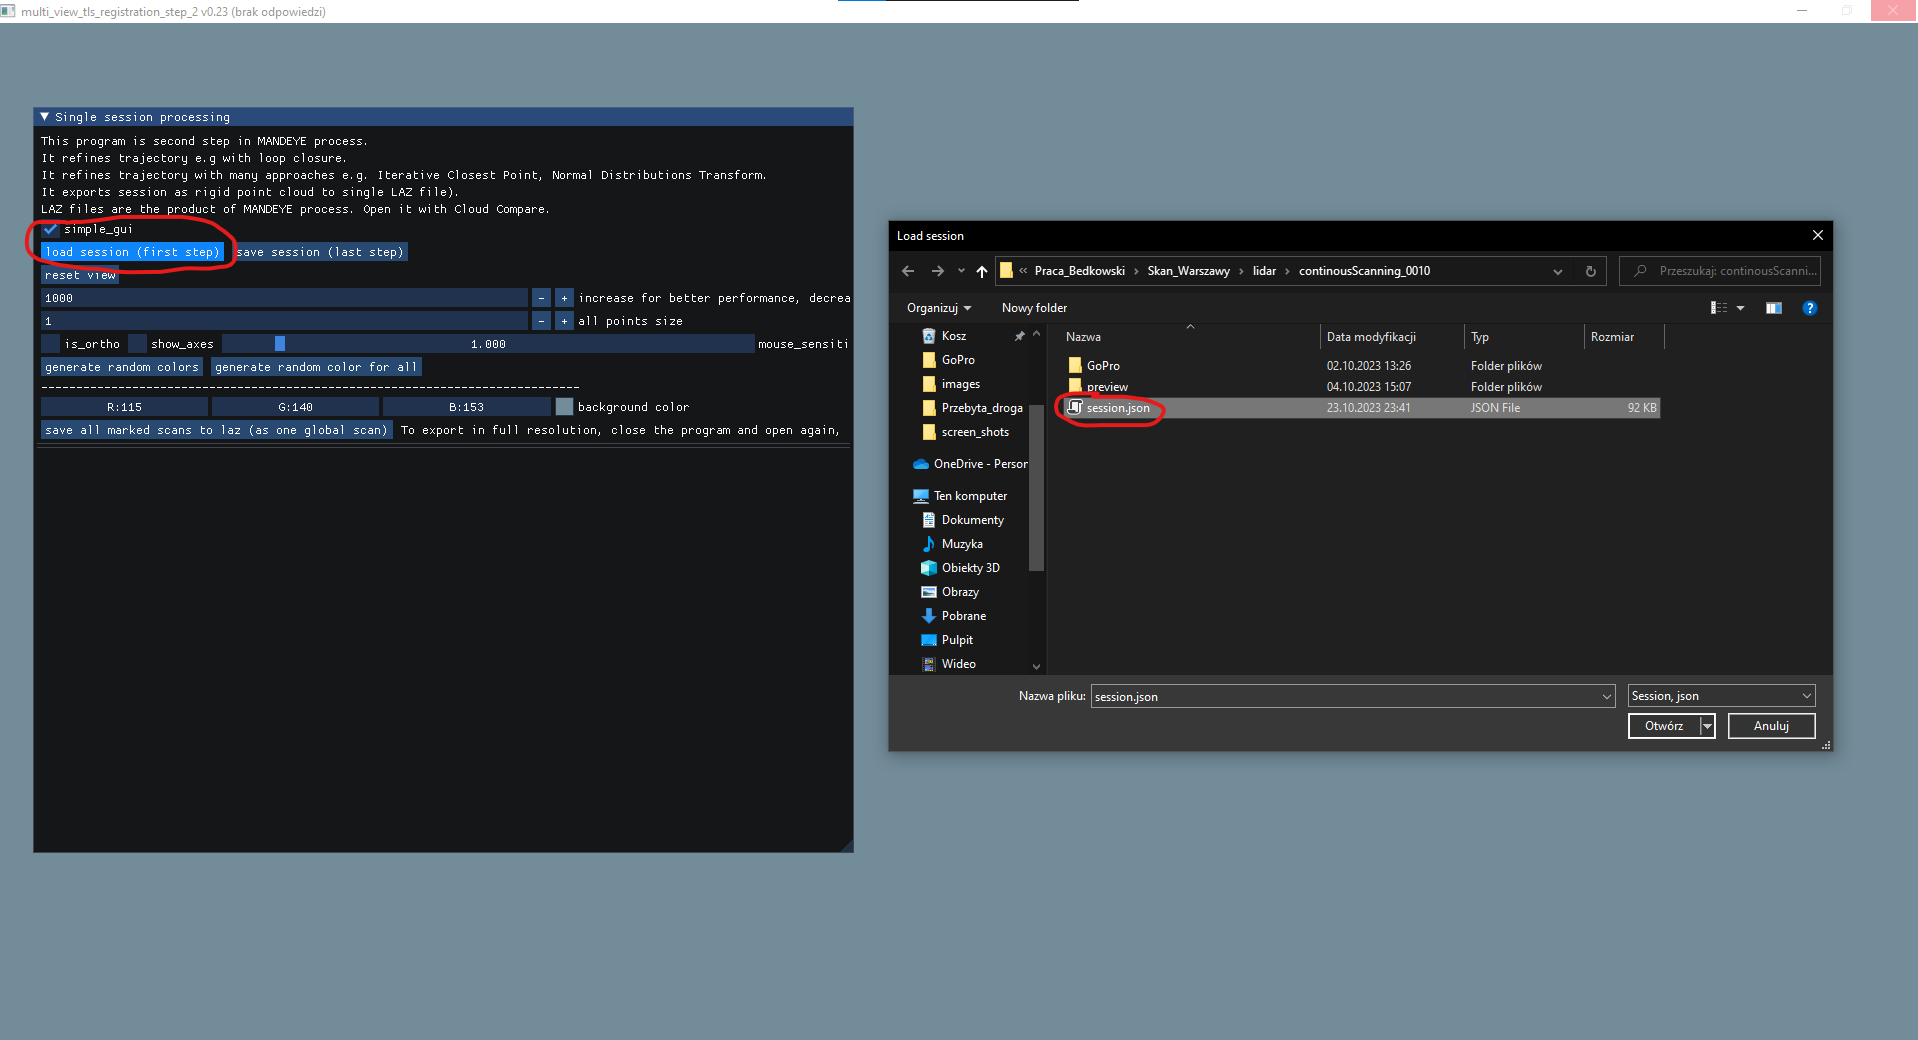
\includegraphics[width=\textwidth]{10.png}
	\caption{Import files prepared by 'Lidar odometry'.}
	\label{fig:10}
\end{figure}

\begin{figure}
	\centering
	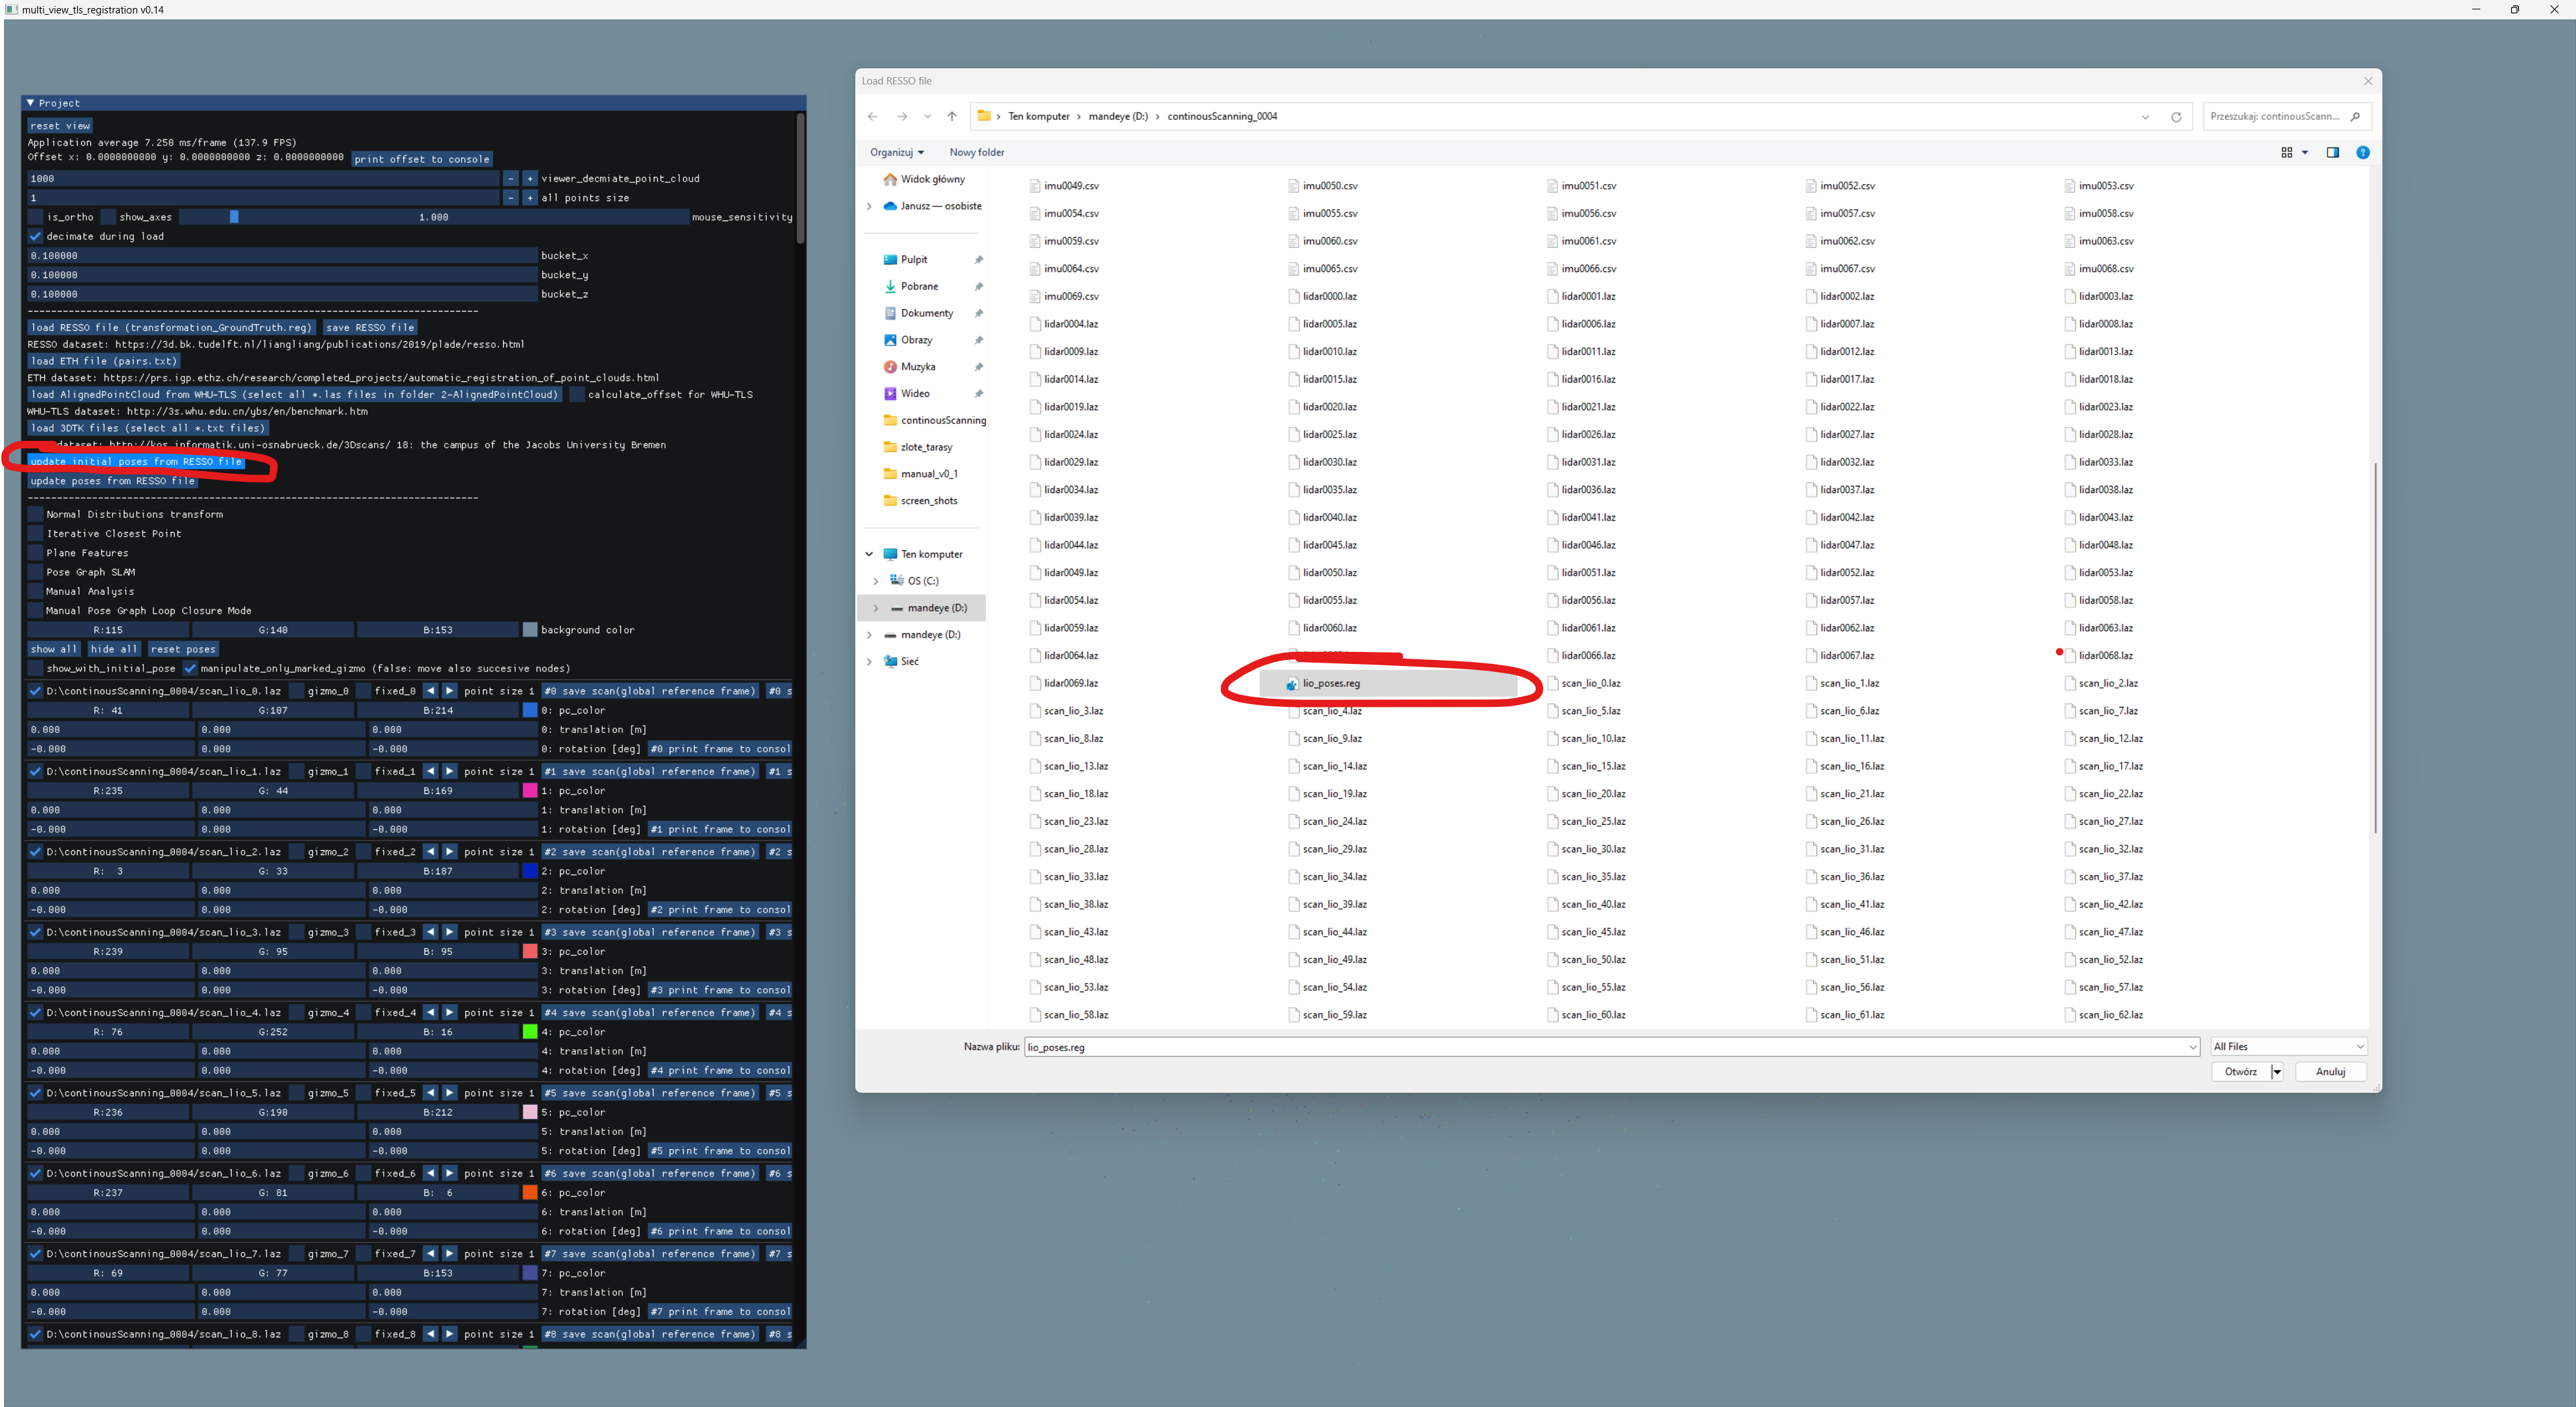
\includegraphics[width=\textwidth]{11.png}
	\caption{Update initial poses from *.reg file.}
	\label{fig:11}
\end{figure}


\begin{figure}
	\centering
	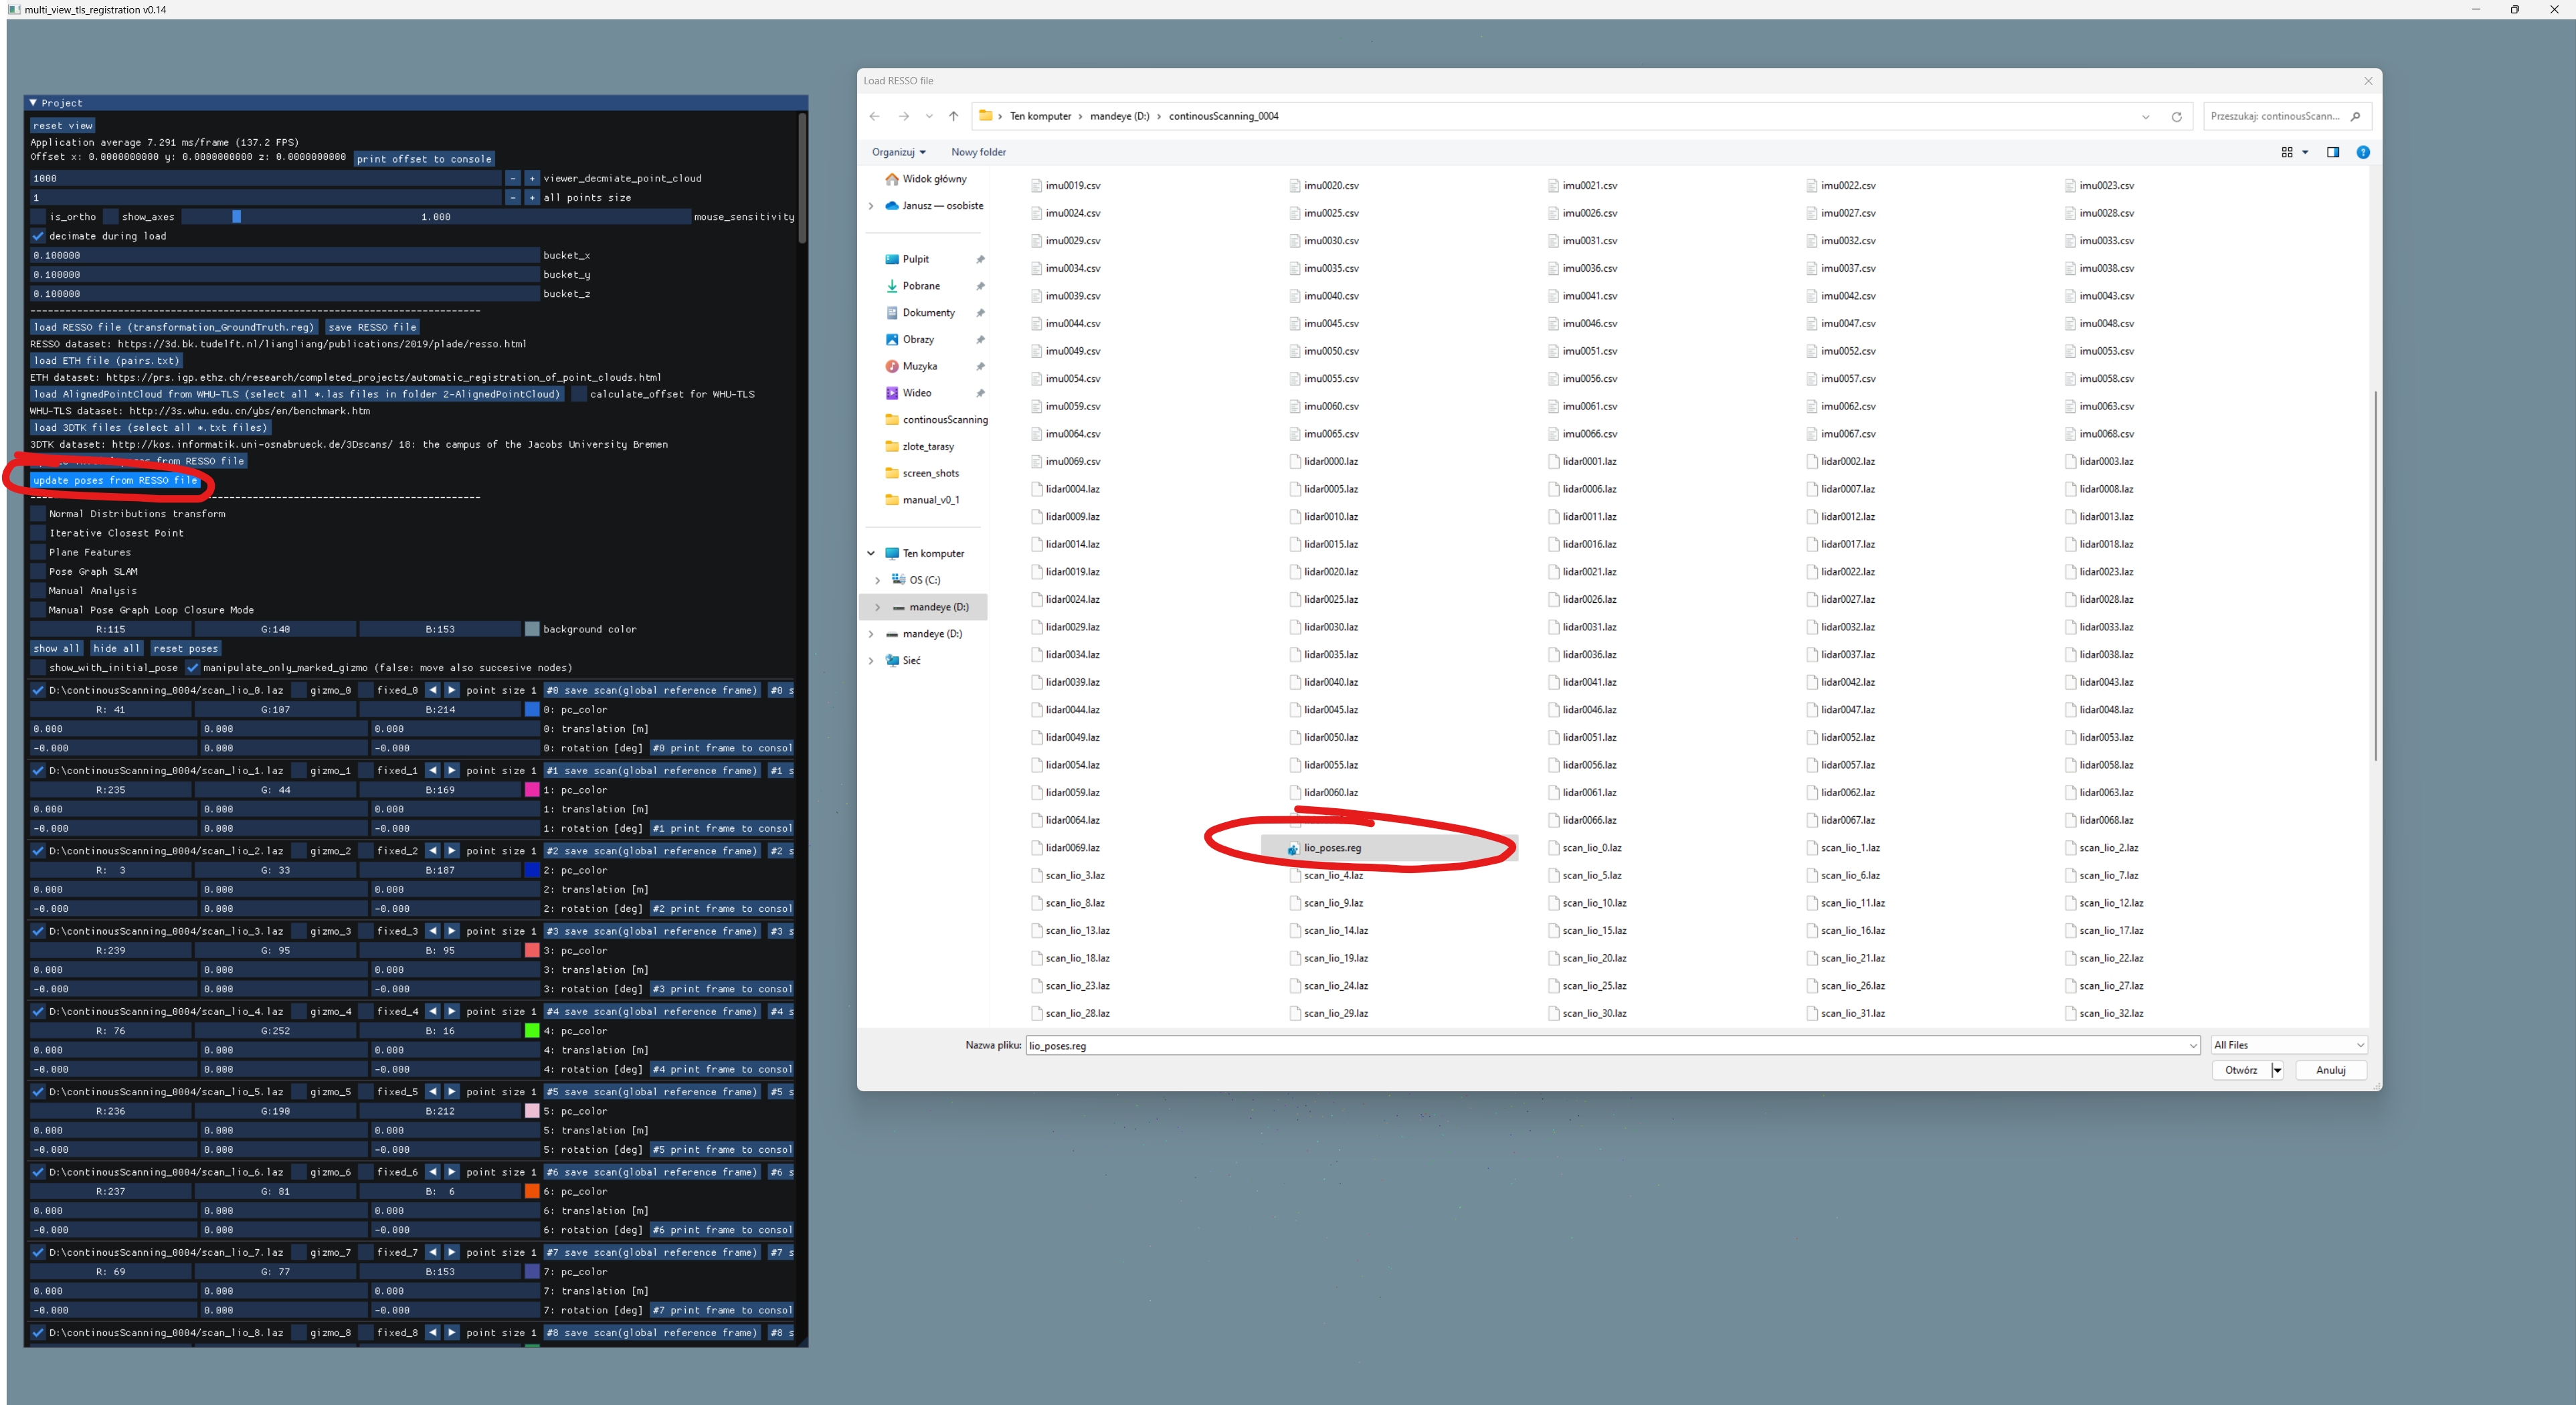
\includegraphics[width=\textwidth]{12.png}
	\caption{Update poses from *.reg file.}
	\label{fig:12}
\end{figure}

\begin{figure}
	\centering
	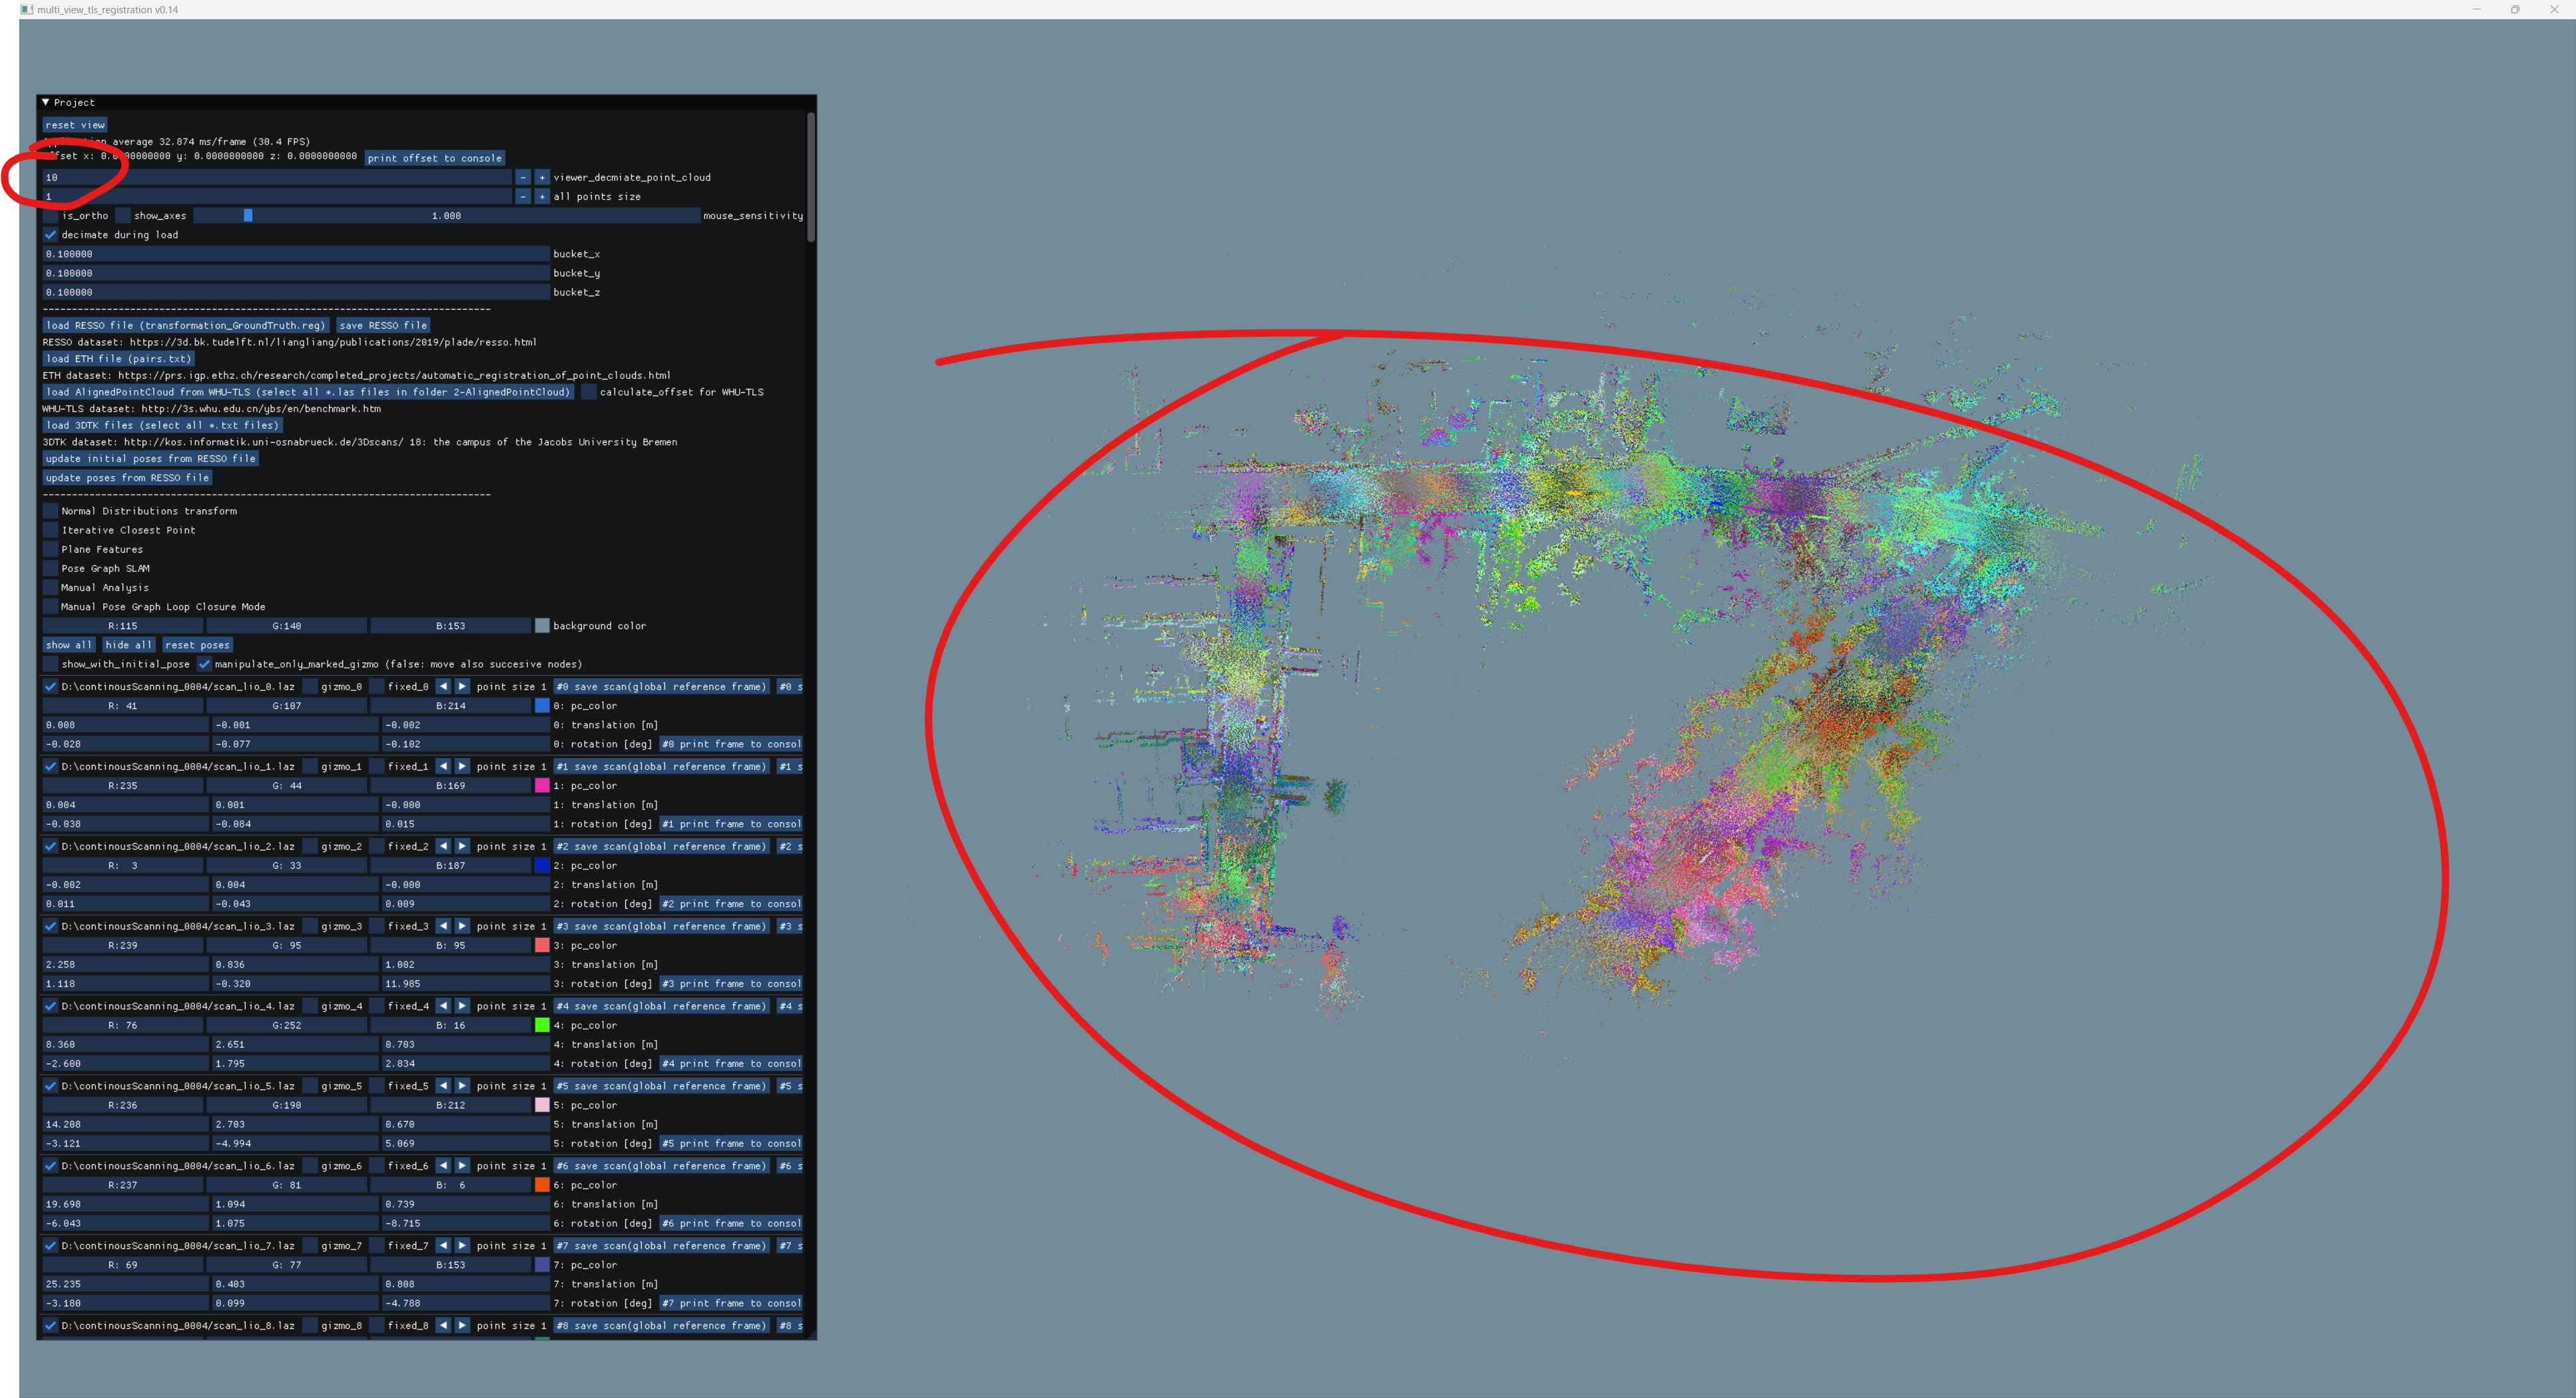
\includegraphics[width=\textwidth]{13.png}
	\caption{Prepare field of view and change decimation to see more points.}
	\label{fig:13}
\end{figure}

\begin{figure}
	\centering
	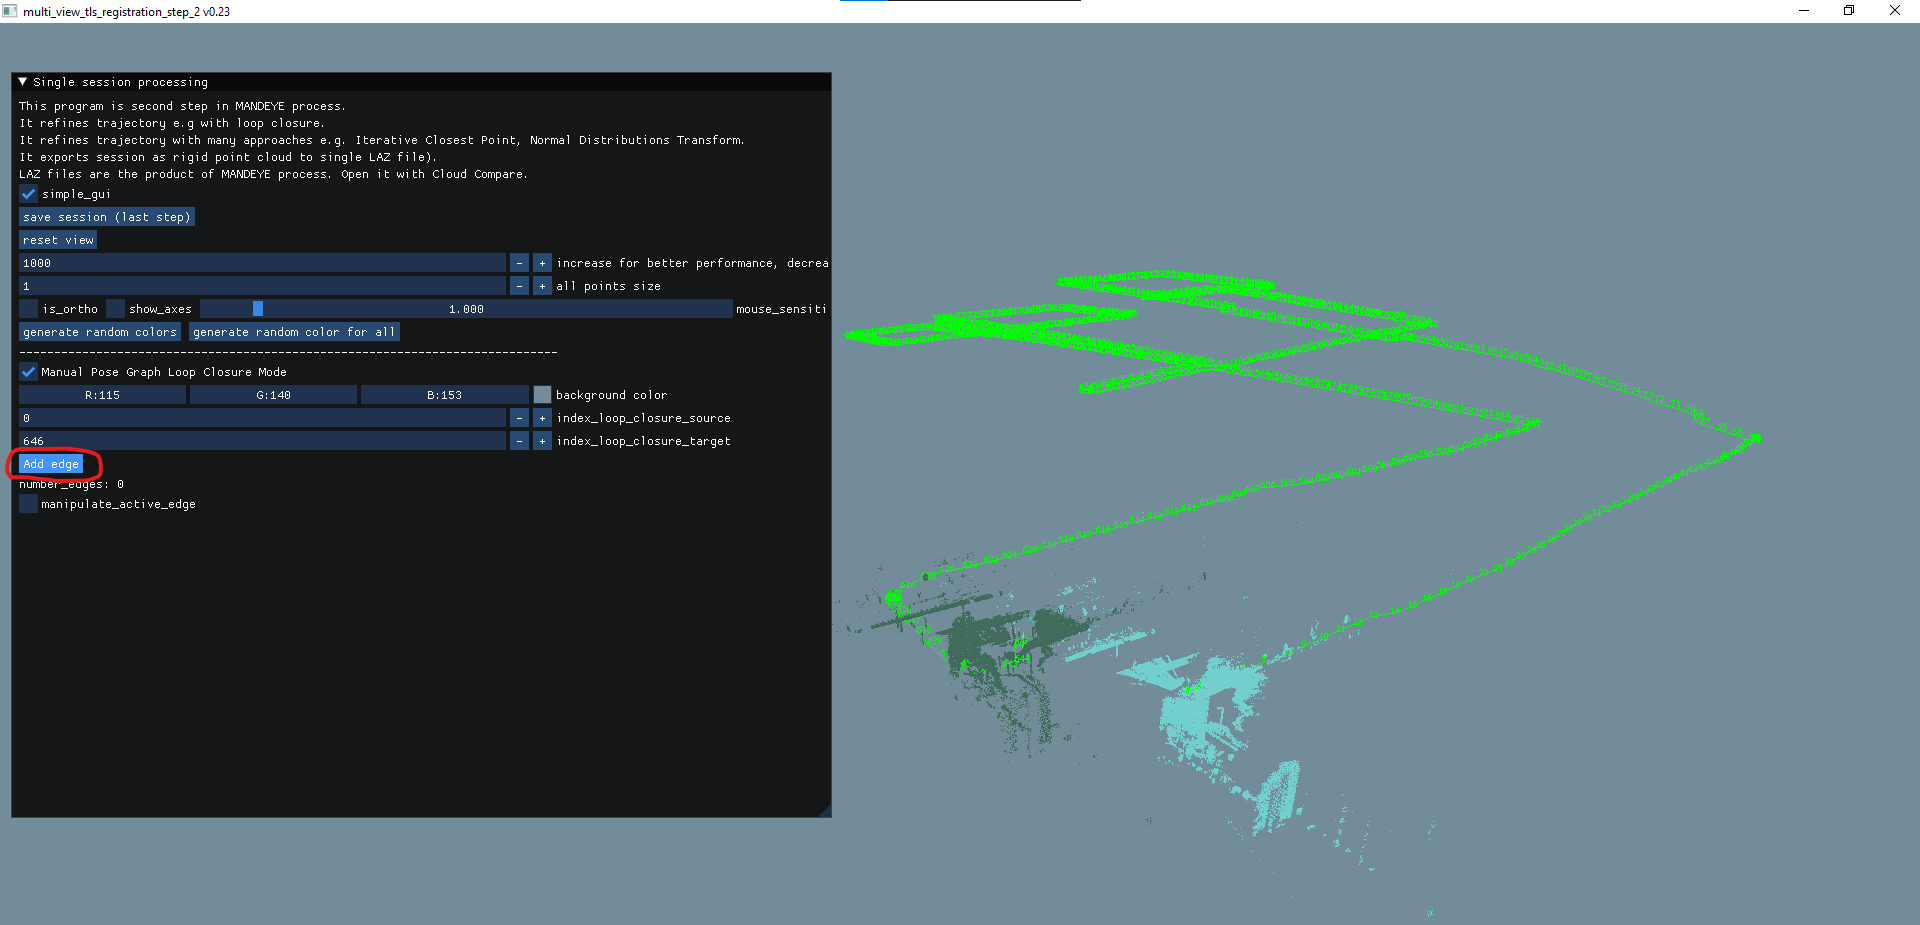
\includegraphics[width=\textwidth]{14.png}
	\caption{Turn on manual loop closing mode and choose two different scans that are not close enough. Add edge.}
	\label{fig:14}
\end{figure}


\begin{figure}
	\centering
	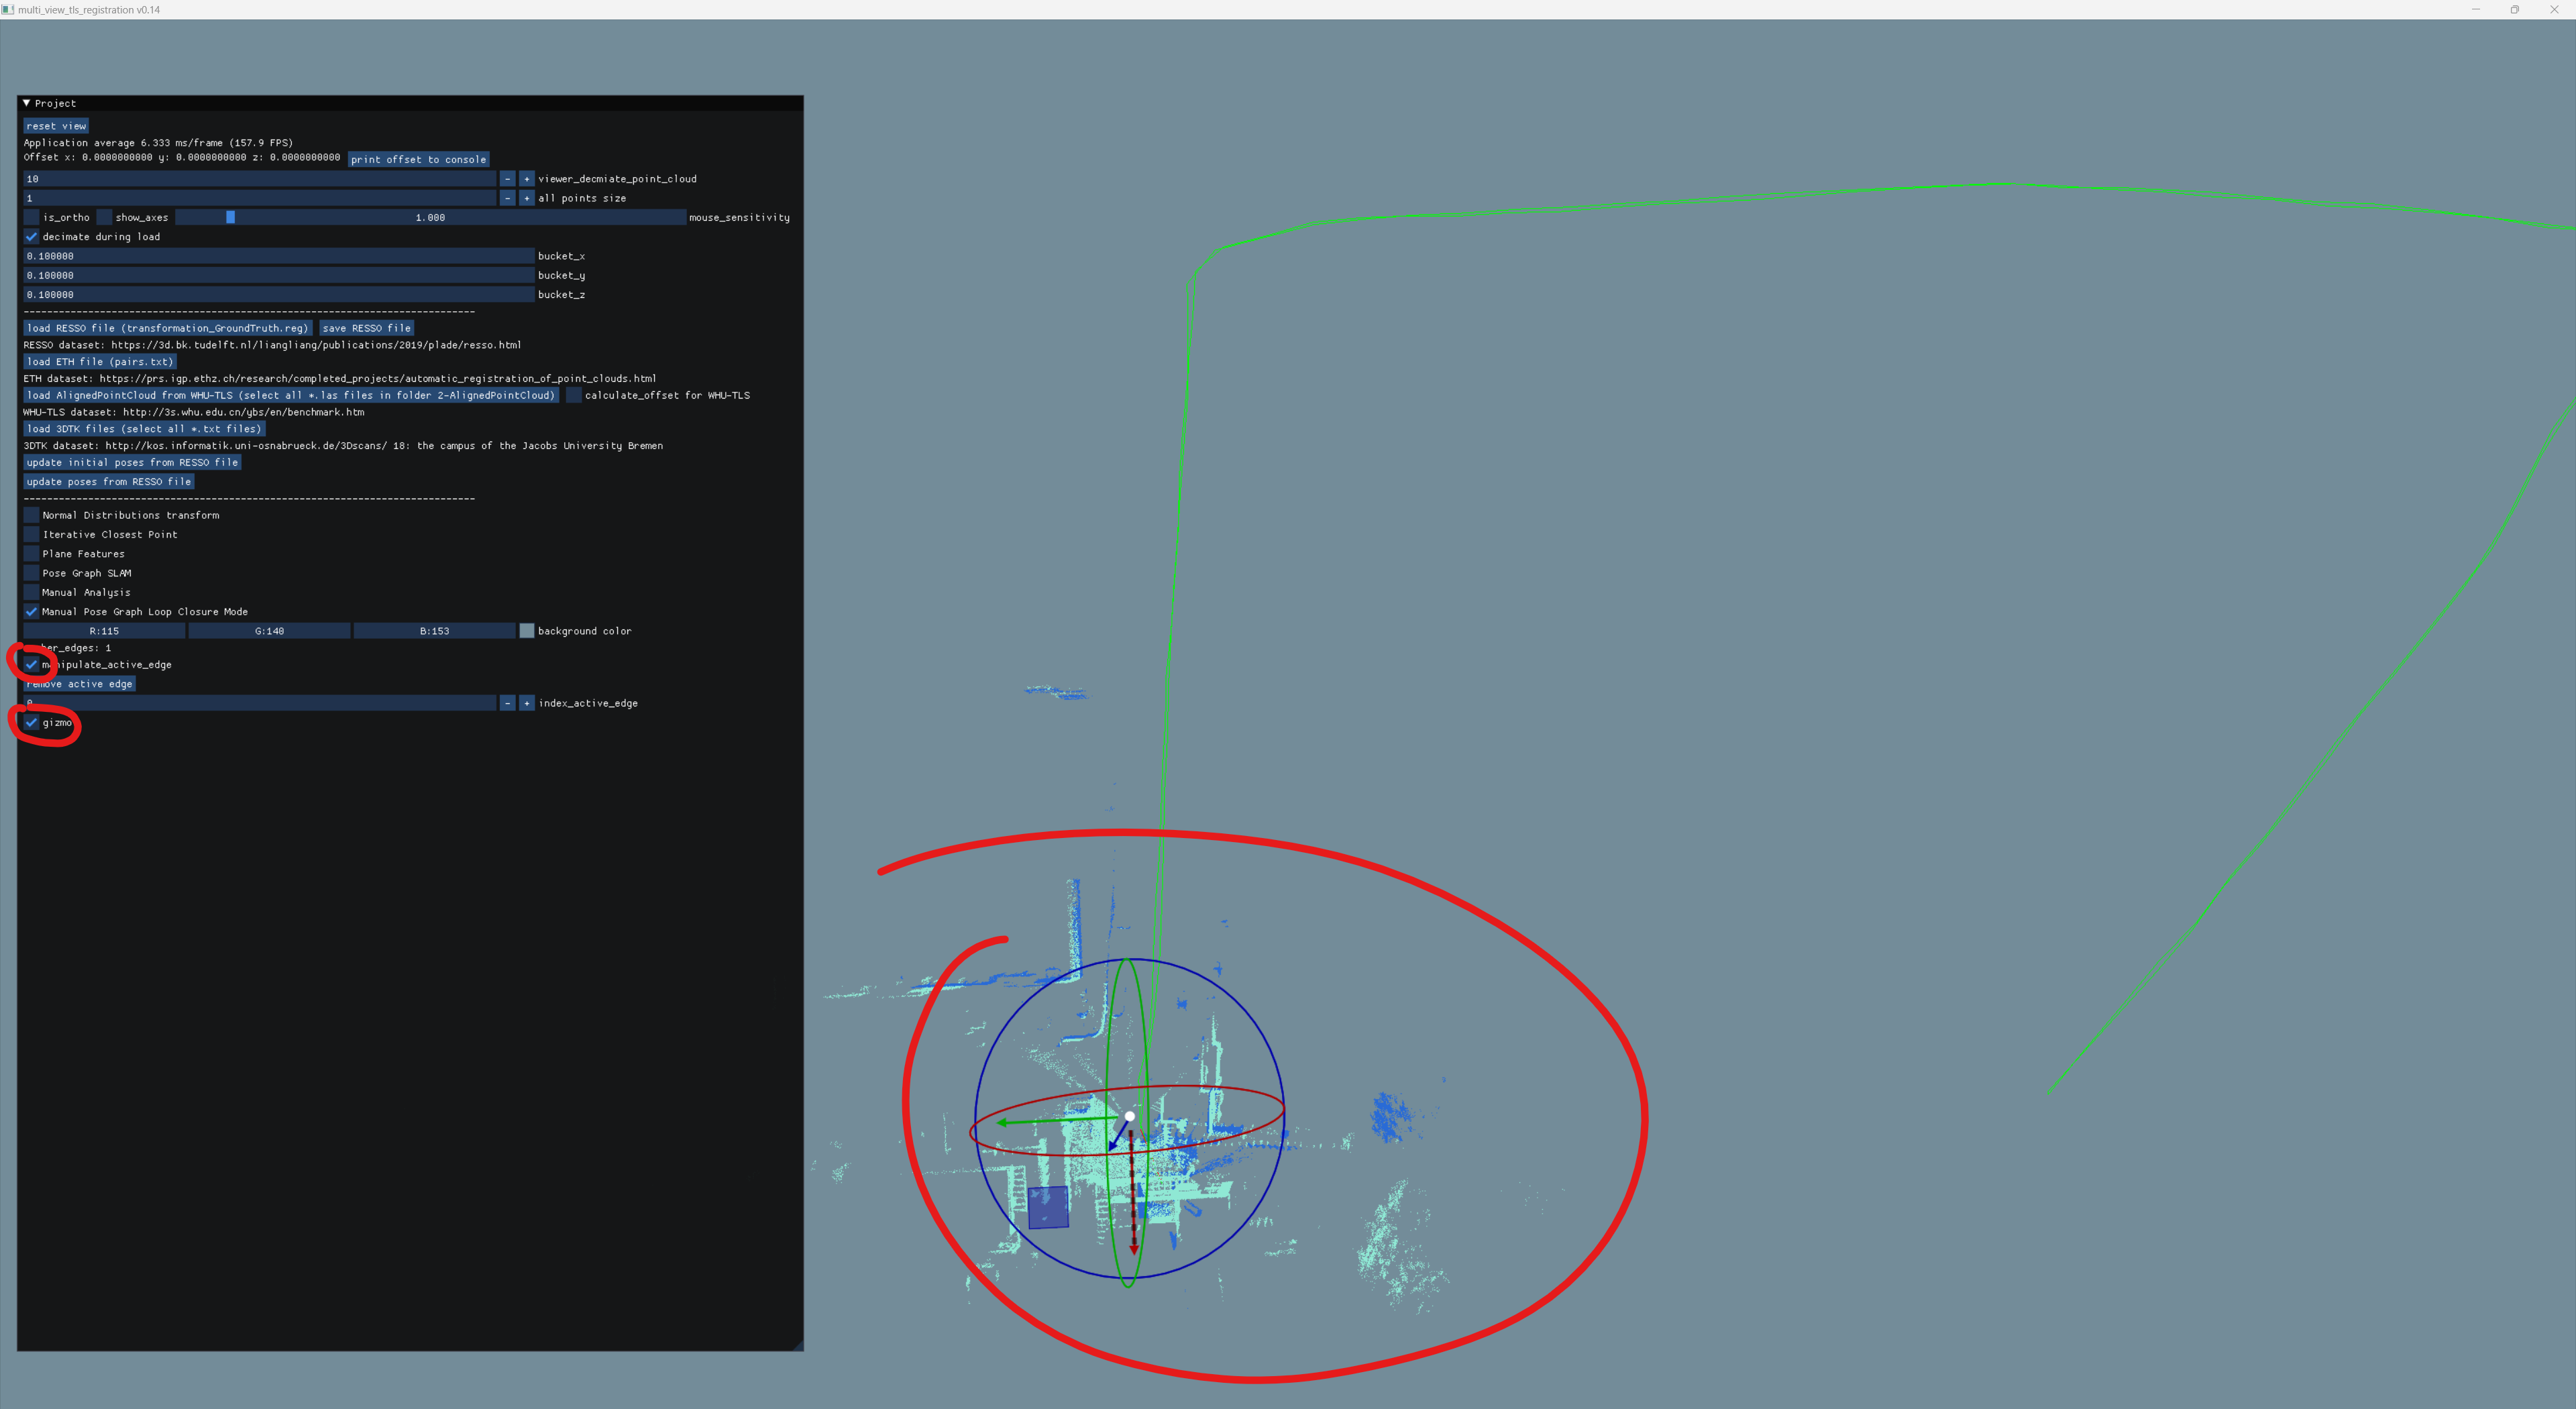
\includegraphics[width=\textwidth]{15.png}
	\caption{Turn on manipulate active edge, turn on gizmo and align scan to scan manually.}
	\label{fig:15}
\end{figure}

\begin{figure}
	\centering
	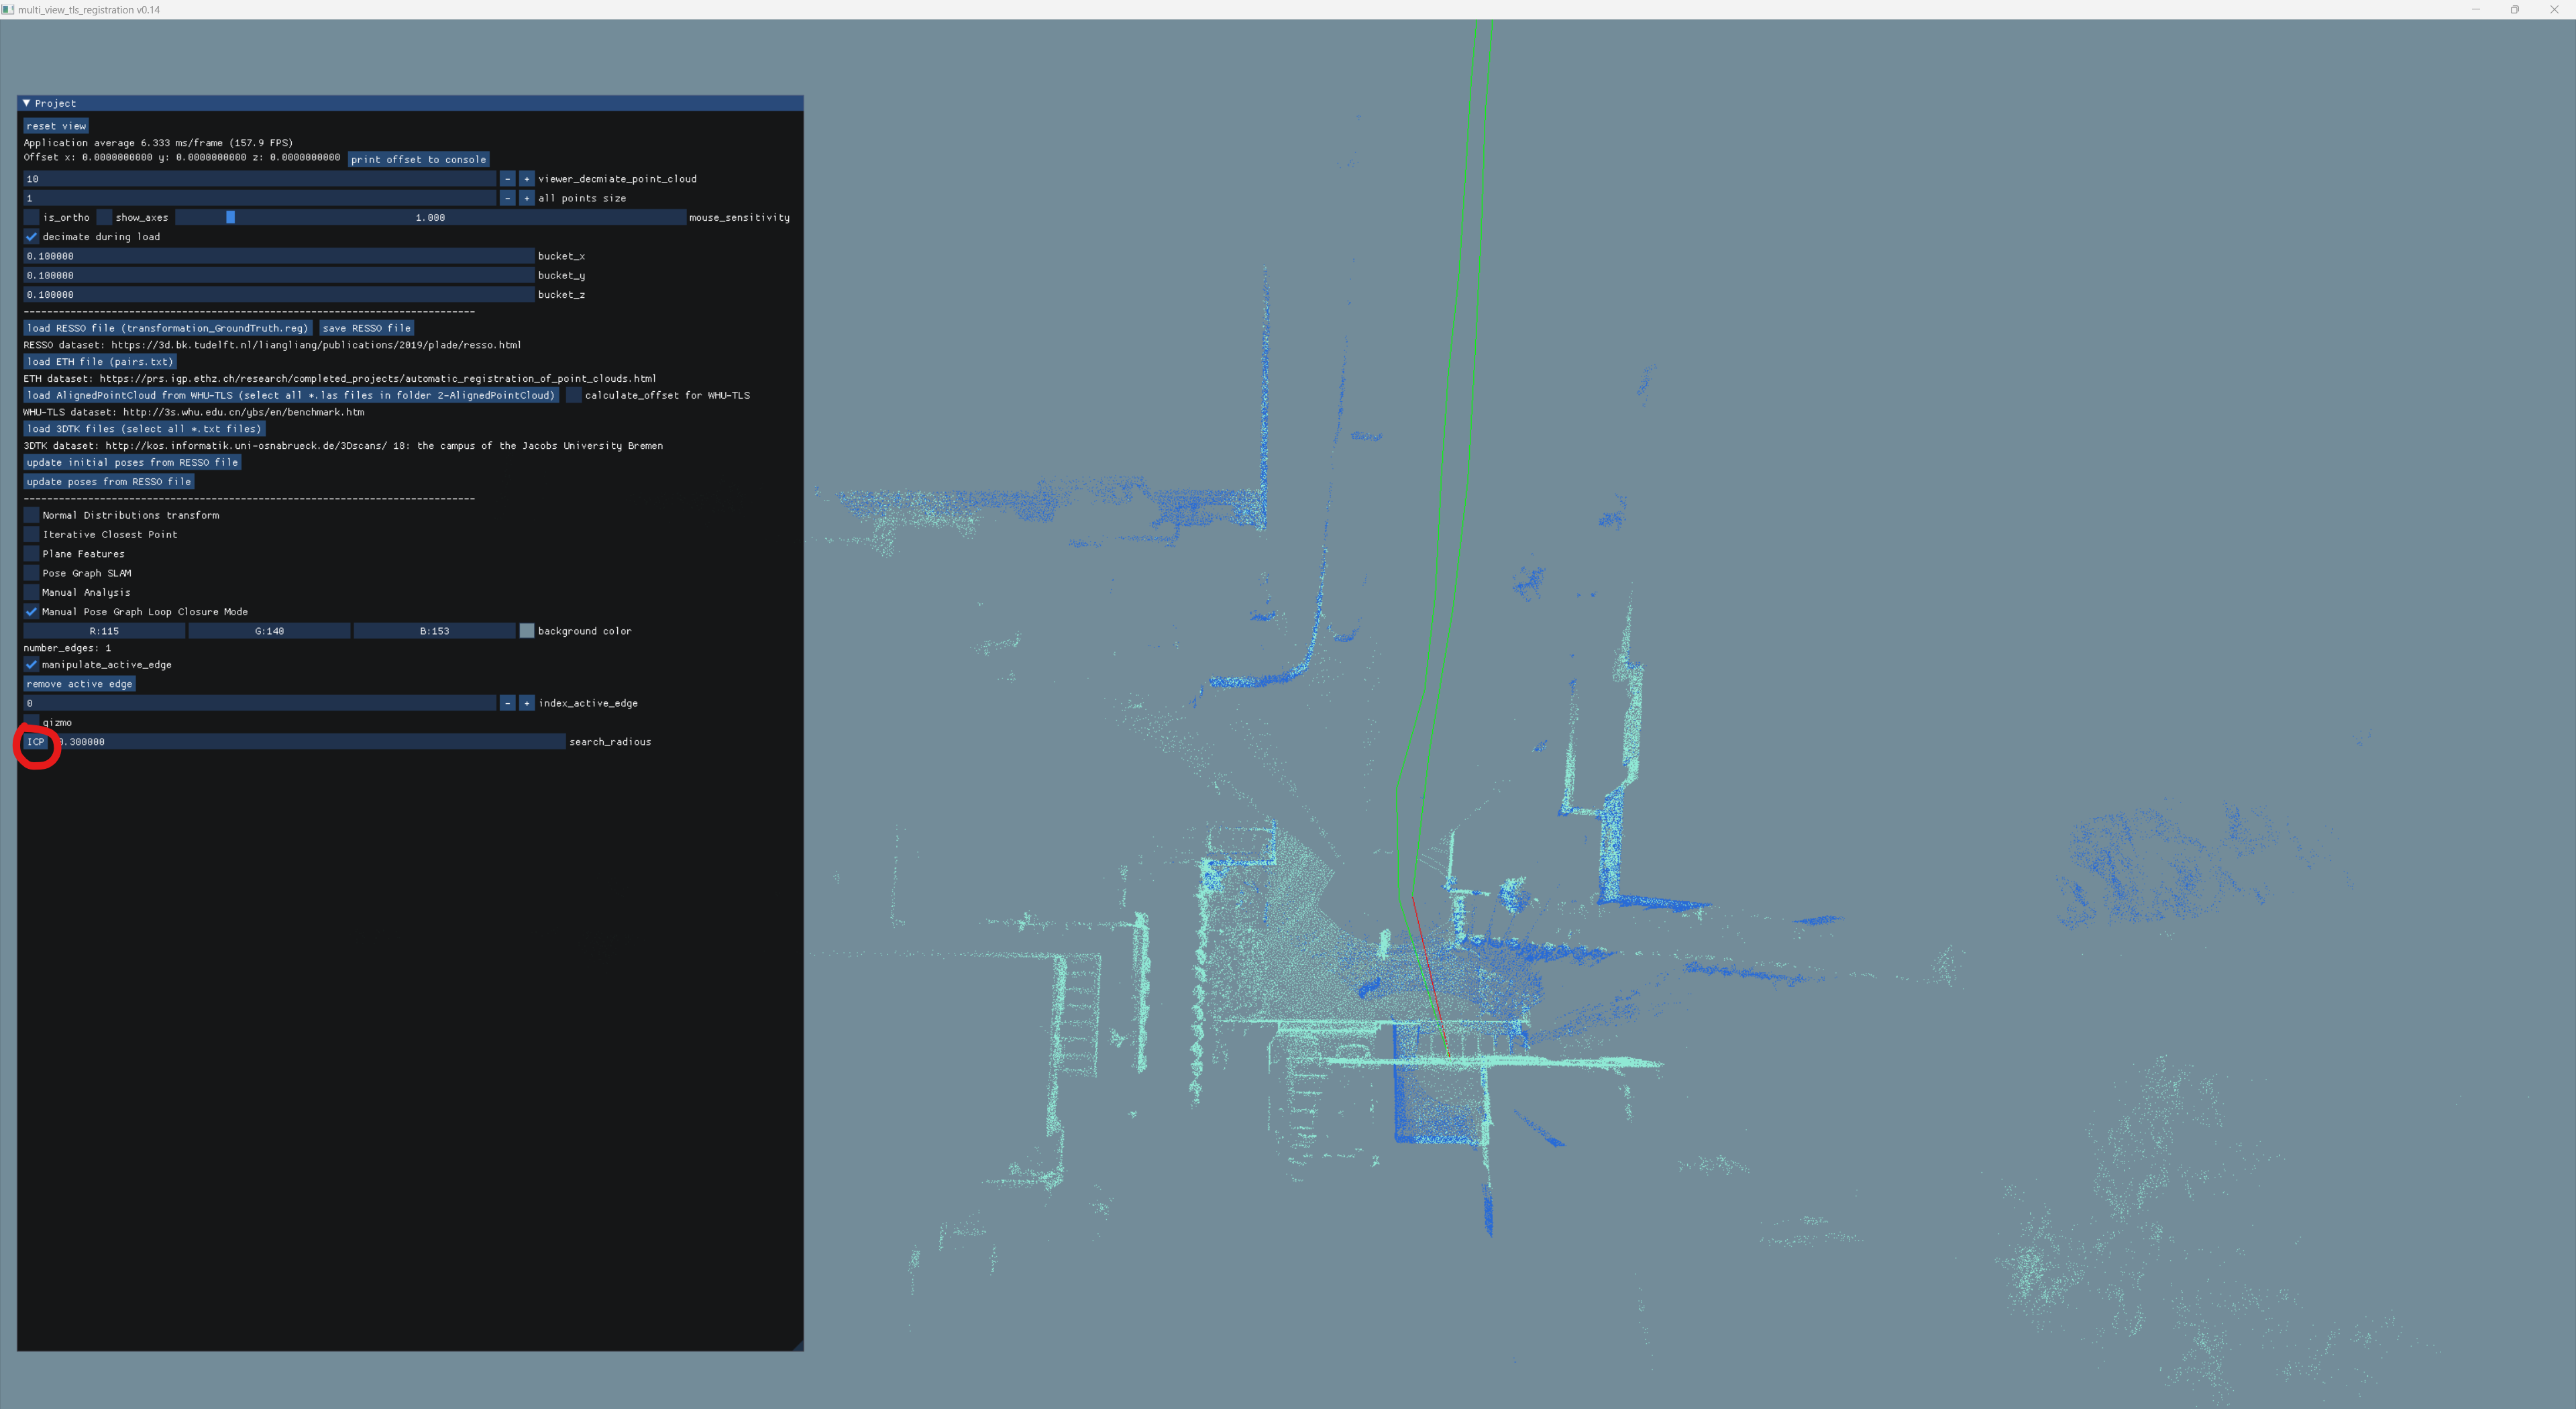
\includegraphics[width=\textwidth]{16.png}
	\caption{Once You are not capable align more accurate, then turn off gizmo and use ICP.}
	\label{fig:16}
\end{figure}

\begin{figure}
	\centering
	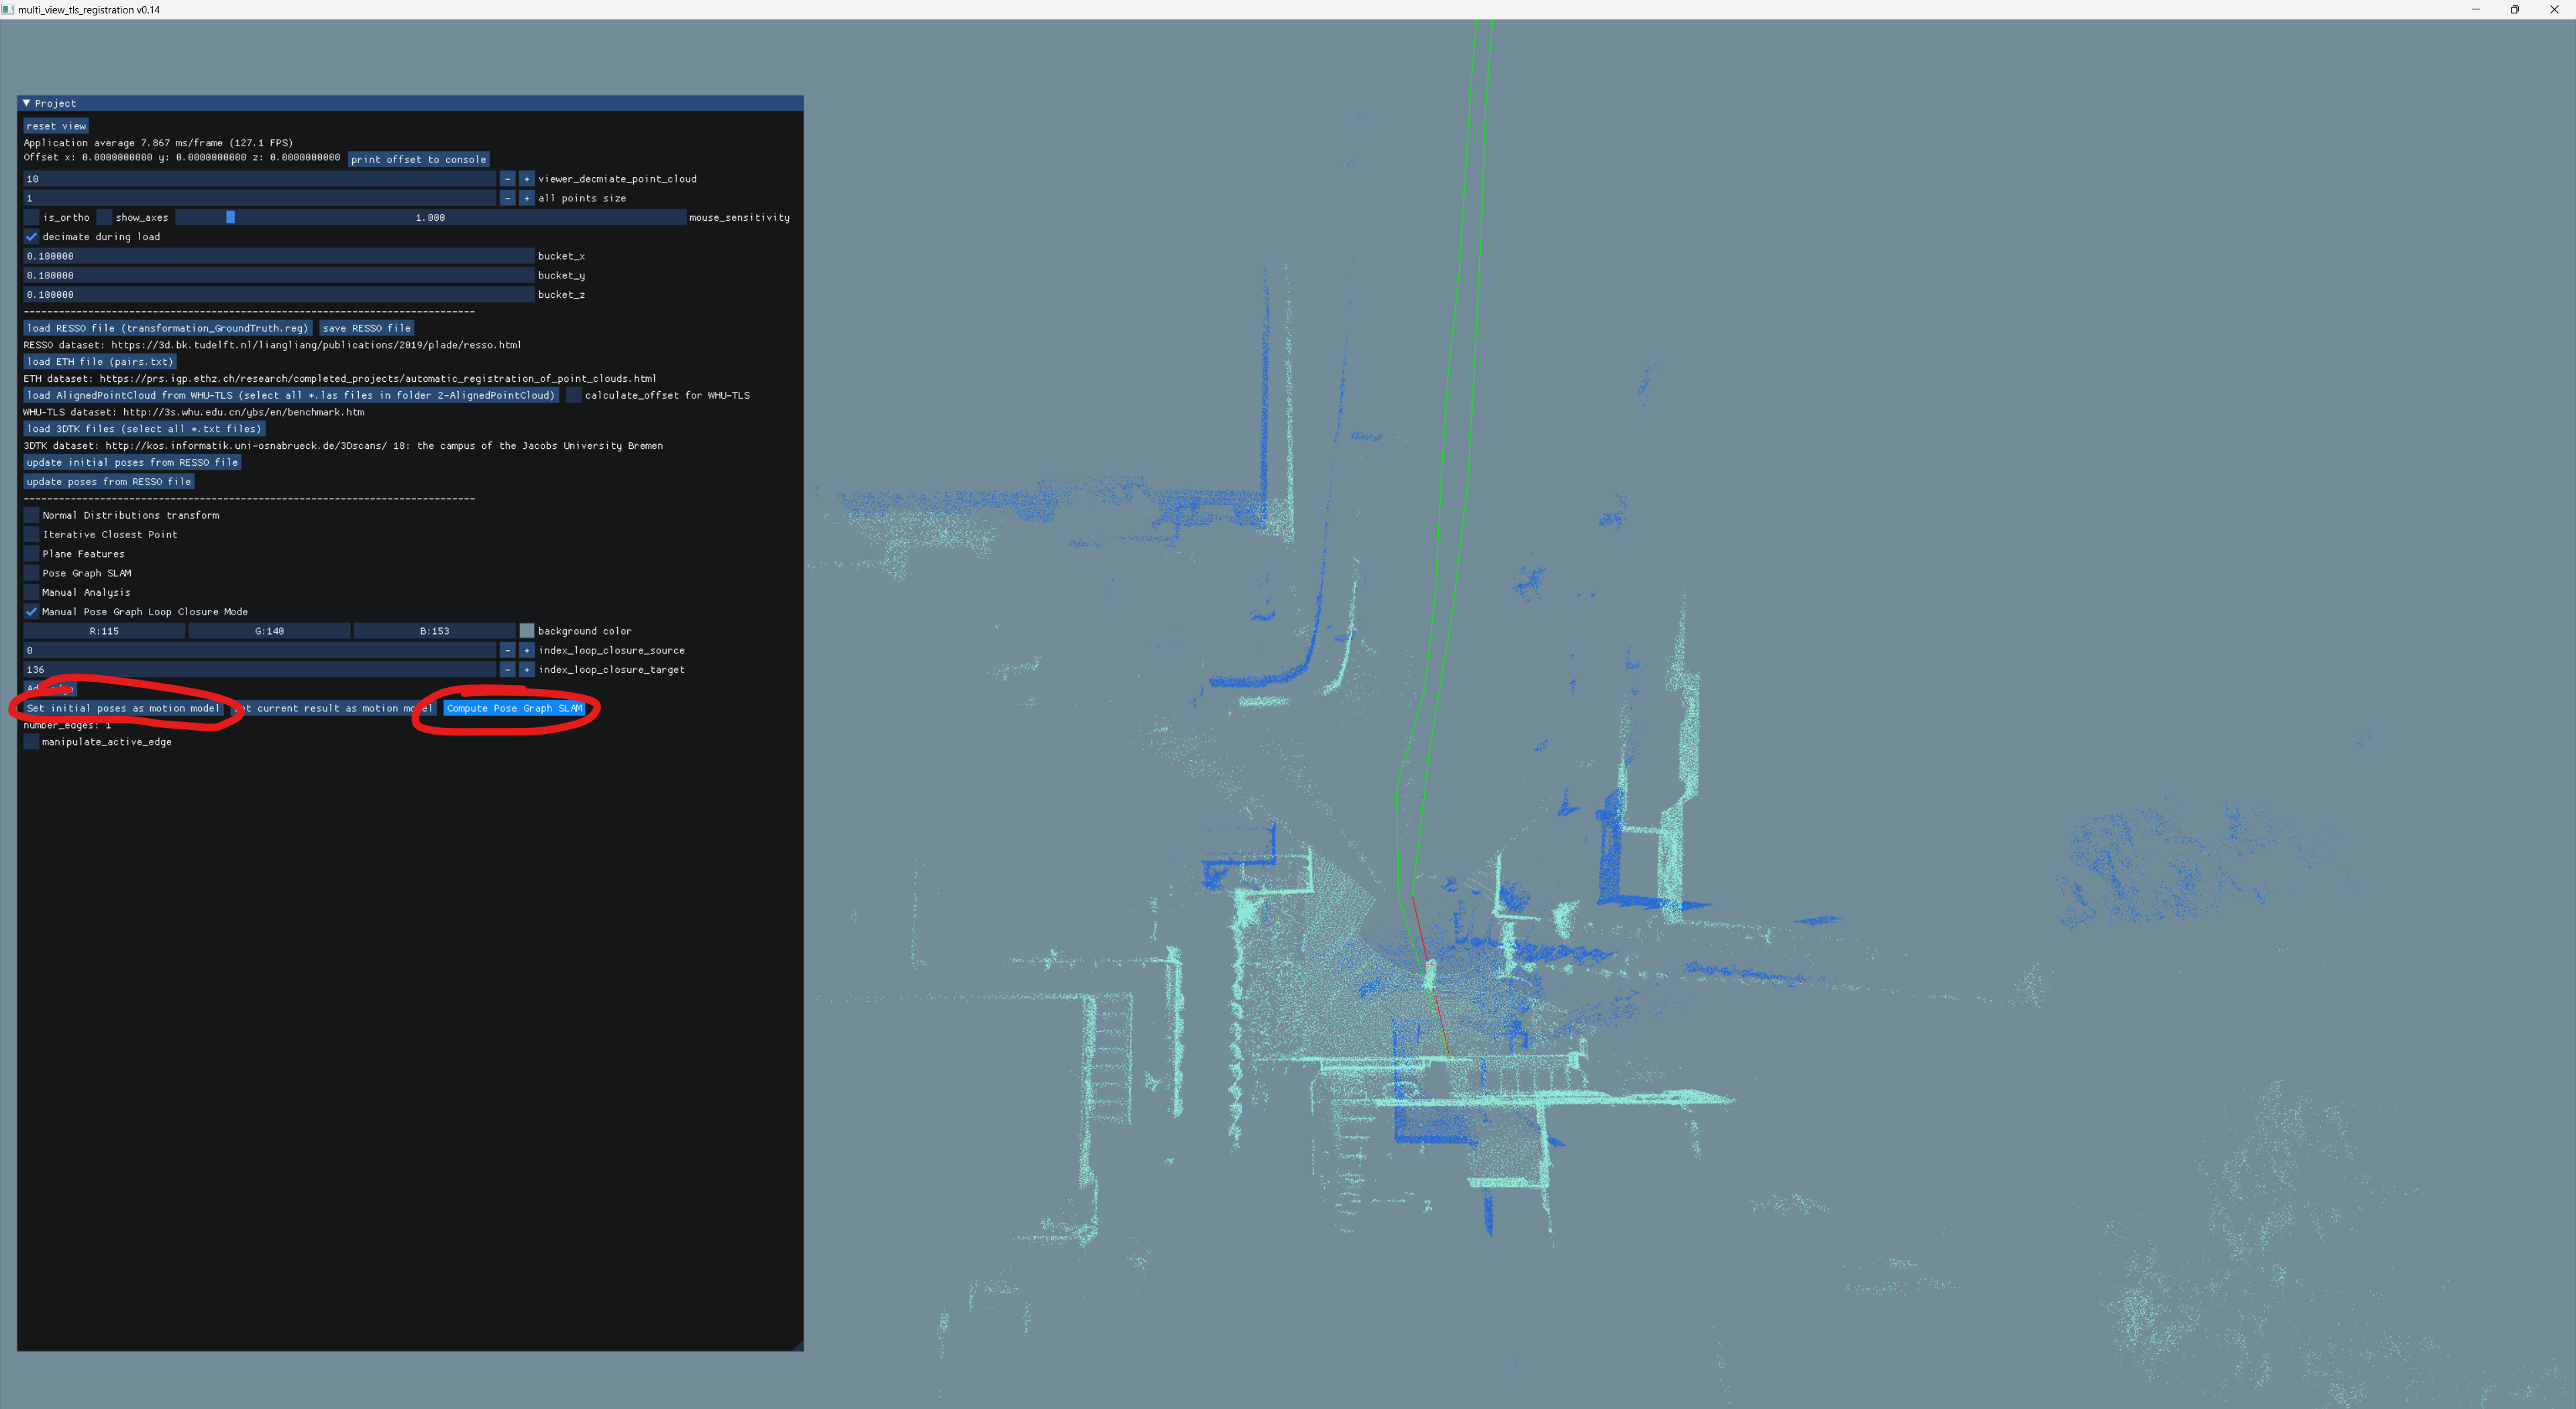
\includegraphics[width=\textwidth]{17.png}
	\caption{Turn off manipulate active edge, set initial poses as motion model, compute pose graph SLAM.}
	\label{fig:17}
\end{figure}

\begin{figure}
	\centering
	\includegraphics[width=\textwidth]{18.png}
	\caption{Turn off manual loop closing mode and inspect if everything ok, if not continue by choosing another pair of scans, refining them and repeat computation of the pose graph SLAM.}
	\label{fig:18}
\end{figure}

\begin{figure}
	\centering
	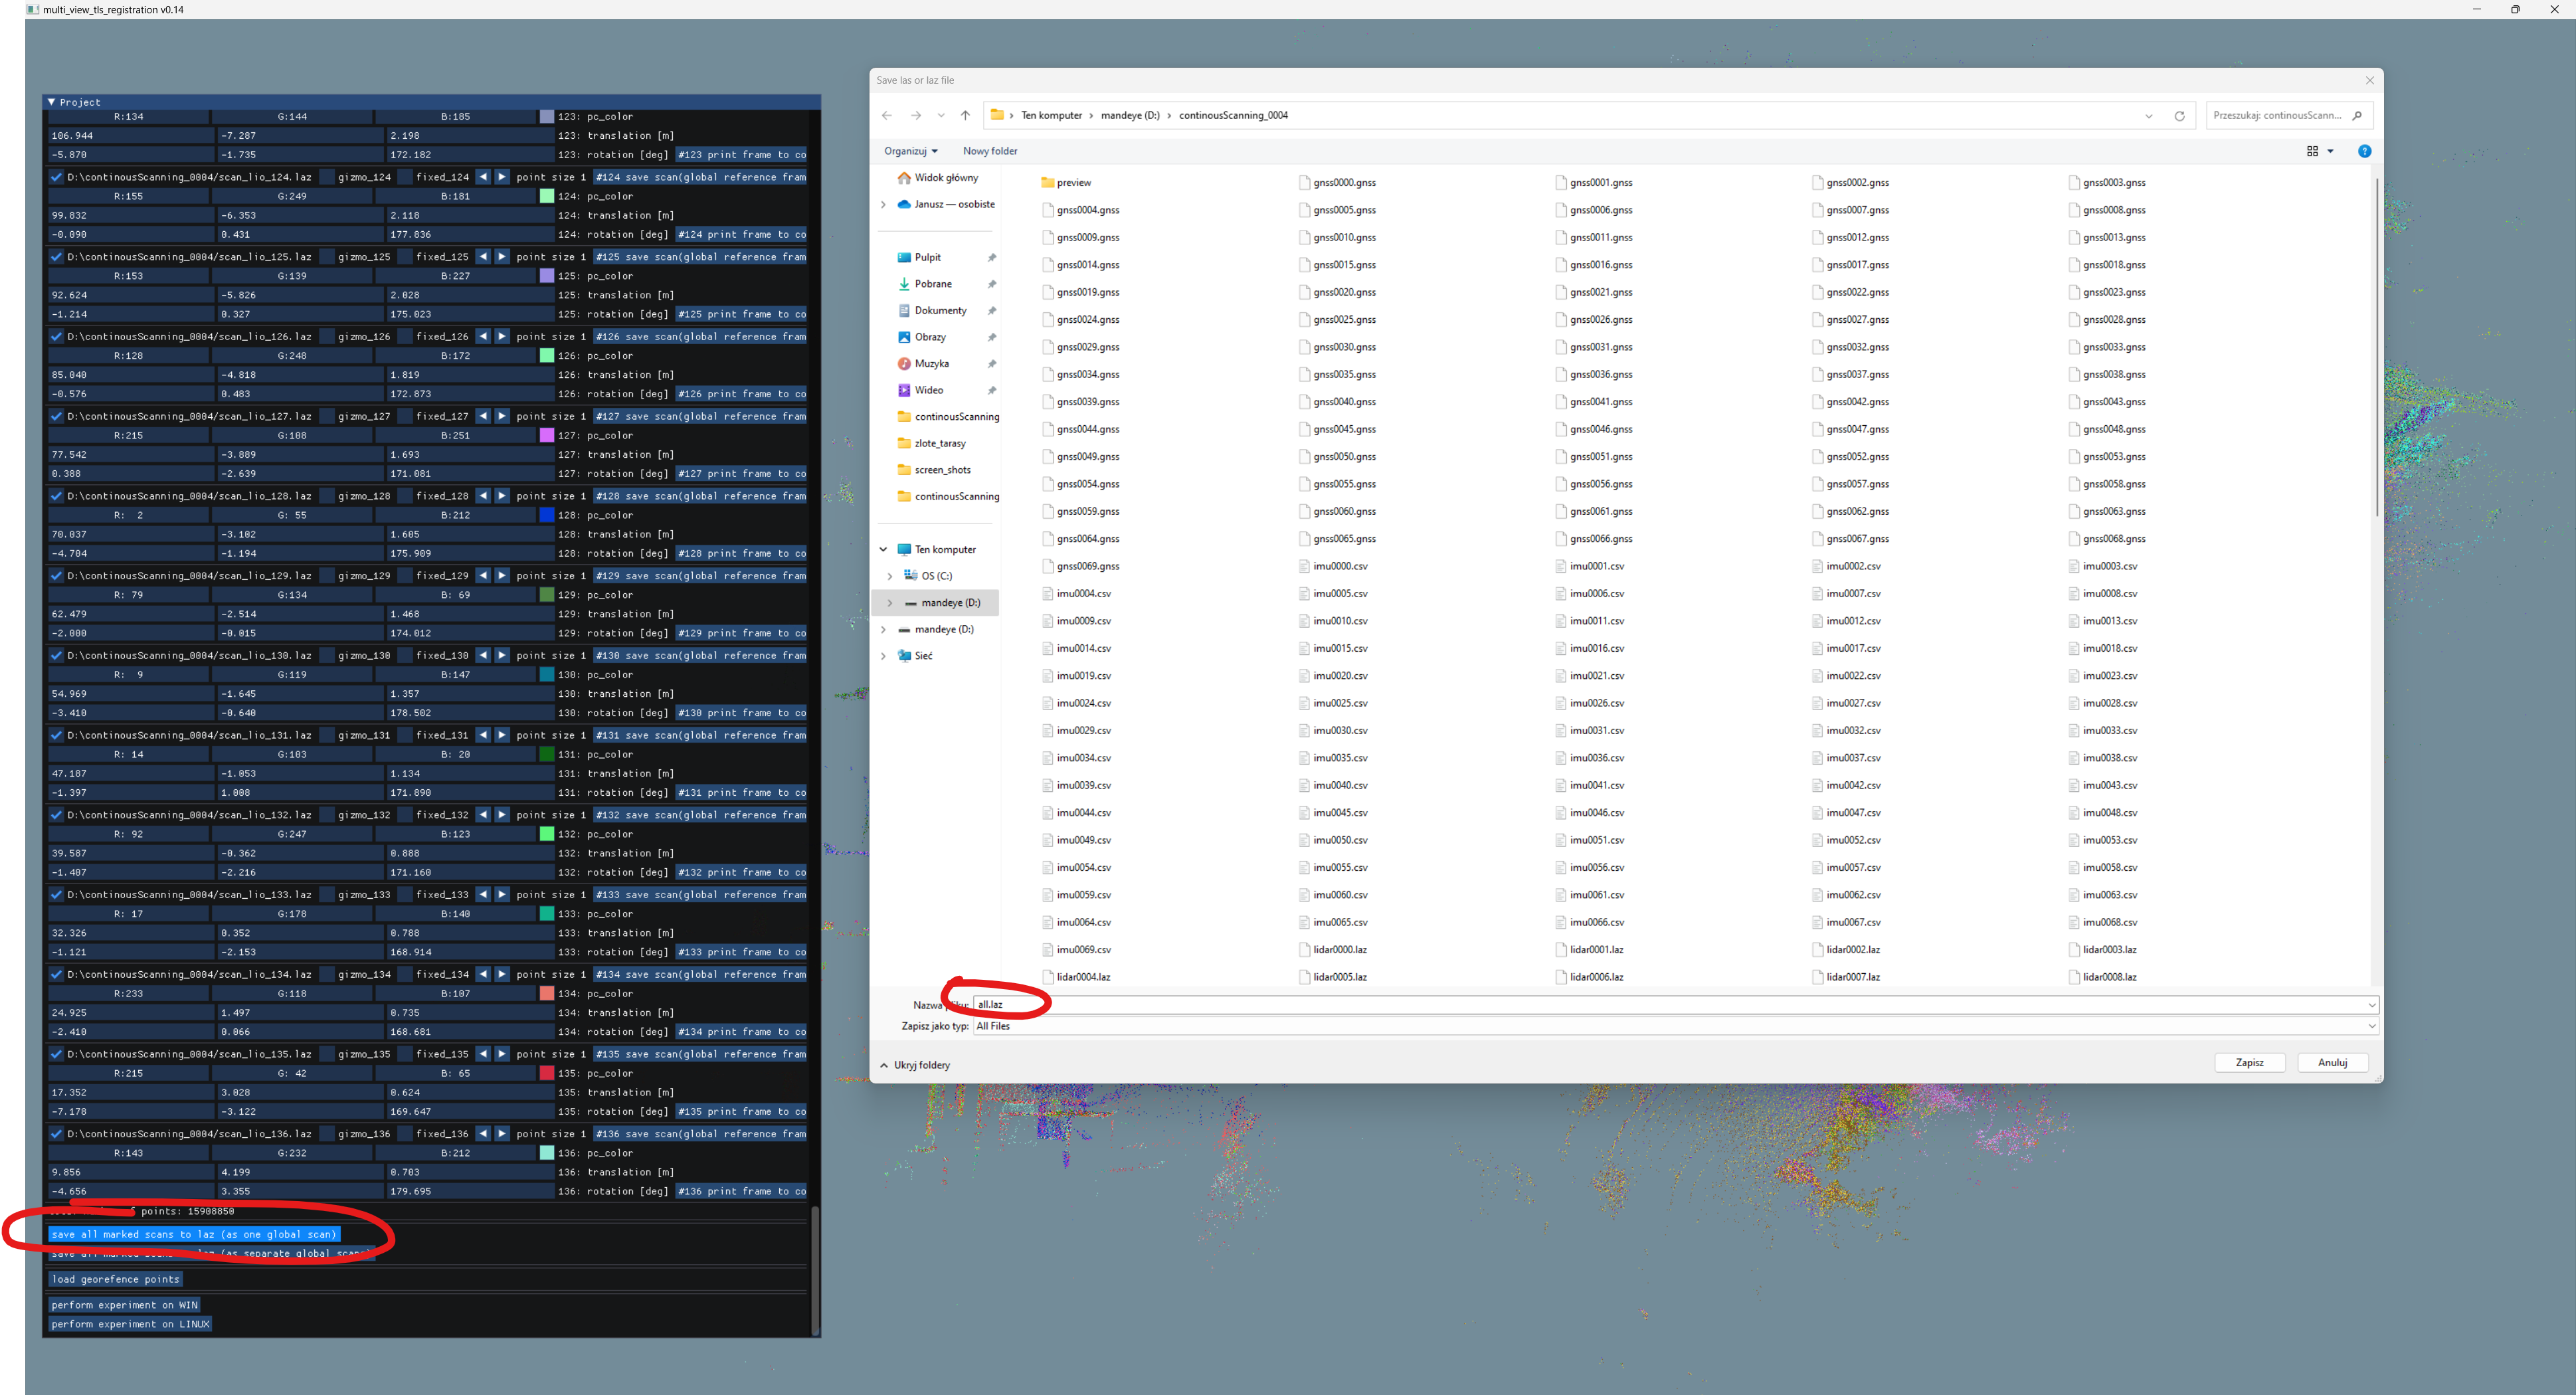
\includegraphics[width=\textwidth]{19.png}
	\caption{Ones the job is thon export data to *.laz. This is Your map that can be loaded by e.g. \href{https://www.cloudcompare.org/}{CloudCompare}.}
	\label{fig:19}
\end{figure}

\chapter{Questions from end users}

\textbf{Do you have recommendations on how to best record data?} \\
I recommend stop/scan mode for most accurate mapping.
Continuous mapping is for increase the time of the survey.  \\
\textbf{How much distance can be between two consecutive start/stop acquisitions?}\\
I suggest not more than 10 meters.\\
\textbf{Do they need to overlap? To which degree?}\\
Stop/scans should be overlapped at least 50\%.\\
\textbf{Continuous scanning: can the sensor change its tilt/angle during the recording phase? 
Or does it assume being in a upright position all the time?} \\
I suggest that MANDEYE  is somehow a upright position all the time. \\
\textbf{How “fast” am I allowed to move (I actually did a rather slow walk).} \\
I was tested it up to 50 km/h\\
\textbf{Can the sensor change height while recording?}\\
Yes.


\backmatter
% bibliography, glossary and index would go here.

\end{document}